
\chapter{利用量子计算机模拟量子化学问题}

在过去的一个世纪,由于在计算过程中采用了很多理论近似,量子化学在研究原子和分子中的电子波函数
以及它们之间的相互作用方面取得了长足的进步\cite{qschem1}。虽然这些方法很独特也很漂亮,但它们基本只能
利用在小系统内。当量子化学面对的系统越来越大,或者要求的精度越来越高时,这些方法,无论是波函数近似或者
密度泛函理论,在新的挑战面前都无能为力。造成这个局面的原因很简单,量子系统的Hilbert空间是随着空间增大而指数增长的,
而经典计算机对于这种指数式的资源消耗是行不通的。

另一方面,量子模拟概念的提出\cite{Feynman}又给解决以上问题开辟了新途径。用量子系统来模拟量子系统,理论上来说
非常完美,经典计算机遭遇的所有计算复杂度问题都可以迎刃而解。自从三十年前Feynman提出量子模拟的思想之后\cite{Feynman},其概念已经
被证明可以处理包括凝聚态物理,原子物理,材料科学,量子化学等很多领域面临的困难问题,本论文的第二章已经对此进行了详细介绍。其中,量子化学的模拟在近些年来发展的尤其迅猛,
目前已经有不少的理论和实验工作\cite{chem1}。

在本章中,我们将从理论上如何利用量子模拟解决量子化学问题出发,继而回顾目前已经在小体系的量子计算机
上实现的演示性实验,包括静态的氢分子能级计算,动态的化学动力学模拟,以及Heisenberg模型的哈密顿量基态问题的求解等。
我们期待在不久的未来量子模拟将成为量子化学研究的重要工具。

\section{量子化学模拟的理论方案}

“\emph{化学家需要精细和缜密,必须杜绝含糊其词的“about”。}”

 \hspace{23em} \emph{--伯齐力阿斯}

或许伯齐力阿斯的名言对于经典化学而言是完全正确的,但可惜的是,对于上个世纪不断发展壮大的量子化学领域,
量子化学家们恐怕不会苟同这句话。

\subsection{量子化学遇到的困难}

量子化学主要的目标是发展理论手段,来尽可能精确地计算分子的性质,以及计算基于量子力学规则的化学反应及演化。
最常见的量子化学处理途径首先是Born-Oppenheimer近似,该近似忽略了电子运动带来的扰动磁场,可以很好地分离电子和原子核的行为。
尽管如此,在这个框架下精确求解薛定谔方程依然是十分困难的,因为计算所需资源随着分子尺寸还是指数增长的。因此,当前发展的经典上的量子化学
处理方法都采用了很多近似。

量子化学中最重要的任务是研究分子的静态性质,包括电子结构,本征能级,振动模式等等\cite{qschem2}。该领域发展出的近似方法主要有平均场Hartree-Fock理论(mean-field Hartree-Fock Theory)以及
各种后Hartree-Fock途径(post Hartree-Fock approach),比如波函数相互作用,耦合簇态,多体微扰理论等\cite{qschem3}。可惜的是,这些高精度的计算方法只能处理小分子系统。密度泛函理论(density functional theory)\cite{qschem4,qschem5,qschem6}
有相对高一些的效率,并且可以在一定精度上应用子在扩大的系统尺度上。线性扩展算法(Linear scaling algorithms)\cite{qschem7,qschem8}对一些特定种类的材料也可以处理拥有几千个甚至更多原子的系统。
以上这些方法,虽然有时可以预言大量子体系的一些性质,但某些情况下它们也会失败\cite{qschem9,qschem10,qschem11,qschem12}。

量子化学中另一个重要的任务是模拟反应动力学。这不仅仅是探索反应机制,更是对化学反应进行引导和控制\cite{qschem13,qschem14,qschem15,qschem16}。利用没有任何近似的传统方法,目前能研究的
化学反应动力学的极限是9个自由度\cite{qschem17}。即使利用不含时的多组态Hartree方法\cite{qschem18},采用很多模型和近似,我们也只能处理大概几十个自由度。如同模拟静态分子能级的情况,
模拟大分子体系的动力学行为目前对经典计算机来说也是无解的。

\begin{figure}[htbp]
            \begin{center}
              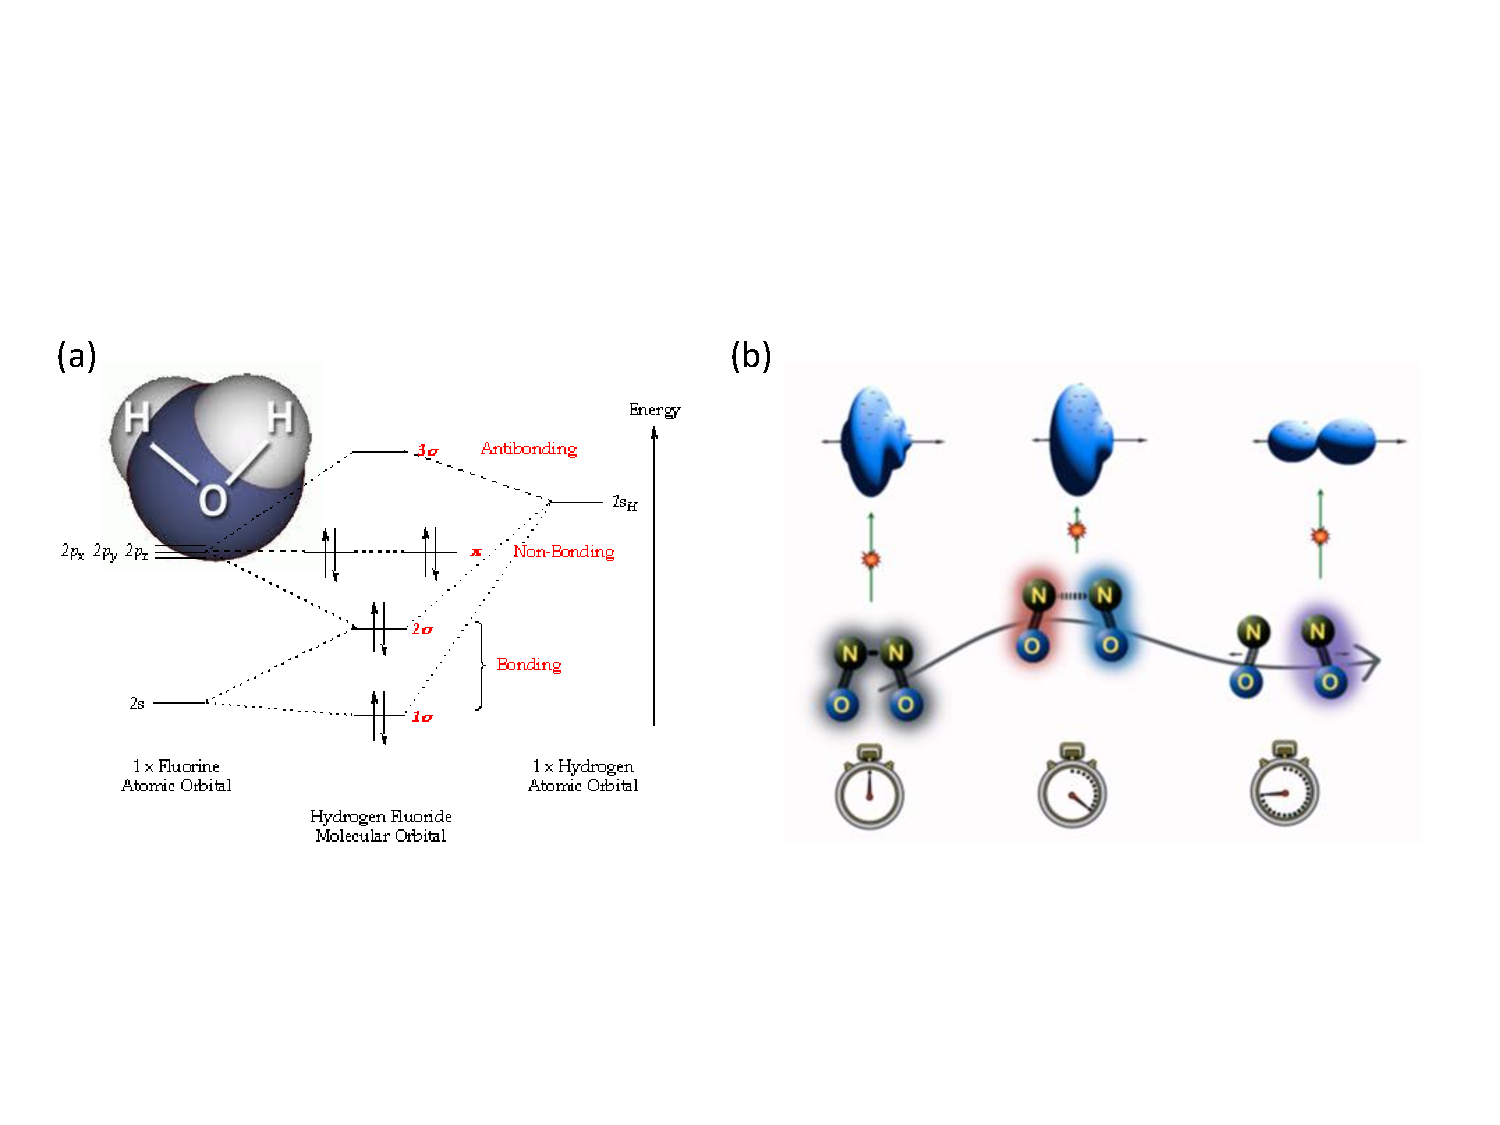
\includegraphics[width= 0.8\columnwidth]{figures/chemscheme.pdf}
              \caption{量子化学面临的两个主要任务。(a) 研究分子的静态性质。(b) 模拟化学反应的动态过程。 }\label{chemscheme}
            \end{center}
 \end{figure}

\subsection{量子化学模拟的一般途径}

本小节我们主要介绍量子化学模拟中用到的方法和技术,主要集中于不远的未来可以或者可能可以用到的部分。

在量子模拟中,我们感兴趣的是量子系统的性质和行为。它们可以是静态的分子,也可以是动态的化学反应。整个模拟过程大致可以总结为三步:

$\bullet$ 把量子态制备到需要的初态;

$\bullet$ 在系统哈密顿量下对初态进行演化;

$\bullet$ 对末态中所需的力学量进行观测。

上面的描述似曾相识,其实这和量子计算的基本过程是类似的。在进行每一步的具体讨论之前,我们先回忆第二章中提到的量子模拟的两种模式:数字量子模拟(DQS)与类比量子模拟(AQS)。
目前,大多数的研究小组关心的是AQS,因为在实验上要实现DQS非常有难度。因此,下面的讨论主要是应用在AQS上的,虽然它们中的部分内容也可以用在DQS上。

(a) \emph{ 初态制备}

原则上说,目前有两种模拟化学系统的途径\cite{chem1}。第一种是二次量子化方法,其中采用了Born-Oppenheimer近似。在这种方法中,
分子中的电子是不能被辨别的,不能作为独立的qubit来使用。二次量子化的优点是它对量子资源的要求并不太高,因为对每种选择的基矢它只要求一个qubit。正因如此,
第一个量子化学模拟的实验正是利用该方法完成的\cite{optics_static}。虽然有优点,但当模拟体系比较复杂而不能用一个简单的基组函数展开,或者模拟对象是一个动力学问题而不能被一个确定的基矢表示的
时候,二次量子化方法就不合适了。为了克服这些问题,研究人员又提出了一次量子化方法。

一次量子化方法并没有考虑Born-Oppenheimer近似。相反地,利用实空间内的薛定谔方程,所有的粒子包括原子核和电子都被放在一起模拟\cite{trotter,qschem19,Polynomial_time_algorithm}。虽然它需要的
资源比二次量子化多很多,但当体系很大时,一次量子化就展示出了自己的优点。由于库仑相互作用是在不同的表象中操作的,二次量子化方法需求
$O(P^5)$个逻辑门,$P$为基组的维度,而一次量子化方法需要$O(Q^2)$个逻辑门,$Q$为粒子数。对多于4个原子的体系,一次量子化方案是更加适合来模拟化学反应的\cite{Polynomial_time_algorithm}。

(b) \emph{ 幺正演化}

当前,我们选择利用Trotter公式\cite{trotter}以及它在高维的扩展\cite{qschem20,qschem21}来实现系统哈密顿量下的幺正演化。假设这个系统的哈密顿量可以被
分解为$H = \sum_{m=1}^MH_m$,那么演化的幺正算子则为$U(t) = e^{-iHt}$。一般来说这个幺正算子的拆解是非常困难的,但利用一阶Trotter公式以及非常小的时间间隔,
我们能够得到
\begin{eqnarray}
 U(\delta t) & = & e^{-iH\delta t} = \prod\limits_{m=1}^M e^{-iH_m\delta t}+\mathcal {O}(\delta t^2)\nonumber \\
 & \approx & \prod\limits_{m=1}^M e^{-iH_m\delta t}.
\end{eqnarray}
模拟的精度还可以通过选择更小的时间间隔$\delta t$和更高阶的分解来继续提高,但无论哪个途径都会增加大量
的逻辑门操作。实验中,这会因为每个逻辑门的不完美性而累积误差。

(c) \emph{ 测量读出}

目前来说实验上主要有两种得到末态信息的方法。第一种就是大名鼎鼎的量子态重构(quantum state tomography),它可以得到末态的所有信息。
但是,随着系统尺寸的增加,重构所需的资源是指数增加的,因为我们要读的末态的Hilbert空间是指数增加的。虽然这和量子计算的思想相悖,但在低维度的实验,特别是演示性实验上,
量子态重构仍不失为一种重要的衡量末态保真度的方法。

第二种读出方法叫做相位估计算法(phase estimation algorithm, PEA)\cite{lq7,qschem22,qschem23,qschem24}。通常来说,我们需要的信息都被编码在
末态的全局相位上,因此是不可观测的。利用PEA,我们可以把信息传递到辅助qubit上,然后在辅助qubit上把需要的相位信息解读出来。但是,对辅助qubit的要求限制了PEA在
量子线路中的广泛应用,毕竟在任何量子系统中产生和操控很多qubit都是很具挑战性的课题。

迄今为止,静态分子能级模拟的两个实验都是通过改进版的PEA完成读出的\cite{optics_static,static}。通过迭代PEA过程,我们可以得到很高精度的结果。在模拟反应动力学的
实验中\cite{dynamical},则利用了量子态重构作为读出手段,因为该实验只用到了3个qubit,Hilbert空间的维度足够小。而且,量子态的完全重构可以直接地给出末态的保真度。当然,当体系增大的时候,量子态重构的
方法就不是很适合了,PEA和其他的一些途径\cite{qschem25,qschem26,qschem27,ini2}在系统包含数十个qubit的时候会更加有效。

\section{静态分子能级的模拟}

“\emph{科学的真理不该在古代圣人的蒙着灰尘的书中去寻找,而应在实验中和以实验为基础的理论中去寻找。}”

 \hspace{23em} \emph{--伽利略}

\subsection{模拟分子基态能级的理论方案}

对量子系统来说,其最基本的性质是哈密顿量的本征值和本征态,而对它们的精确求解需要量子算法\cite{lq7}。量子化学中的情况也是类似的,
给定一个分子的不含时哈密顿量,我们第一步的任务就是计算它的基态能级,也就是哈密顿量最小的本征值。在经典计算机中,这是一个非多项式(non-deterministic polynomial, NP)复杂度的问题,所有已知的经典算法都要求
指数的时间复杂度。

另一方面,量子模拟已经被证明可以在多项式时间内有效的解决这个问题\cite{lq7}。利用量子快速傅里叶变换,局域哈密顿量的本征值和本征态可以在多项式时间内被求解,并且原子物理中的很多经典上难以解决的问题可以利用
50到100个qubit的量子计算机解决\cite{lq7}。也就是说,这种尺度的量子计算机就可以超越经典计算机的能力了。最近,NMR上已经完成对Heisenberg自旋模型的基态能级问题的模拟\cite{yexiao}。

具体到量子化学里的分子性质上,Aspuru-Guzik小组在2005年提出了计算分子能级的算法\cite{Alan_first}。与前面提到的算法相比,在该算法中,基态能级的信息被编码到了
相位上,并通过递归的PEA算法测量出来。该算法把需要的读出用量子寄存器从20降到了4。在该方案中,qubit的数目随着基组函数的数目线性增加,而逻辑门的数目则是多项式增加的,因为波函数与qubit之间的直接映射保证整个幺正算子可以被
有效的分解为多项式数目的逻辑门。他们同时认为量子模拟可以在30到100个qubit的范围内超越经典计算的极限。

模拟静态分子能级的过程依然可以分为三步:编码和初始化,受控演化和相位读出。其实这三步就是前面提到的量子化学模拟一般理论方案中的三步,只不过更加具体罢了。

首先是编码和初始化。所有的量子模拟任务首先都需要把系统的波函数通过合适的映射来编码到qubit上,以建立模拟系统与真实物理系统之间的桥梁。对于多粒子系统的波函数来说,它经常用单粒子的原子轨道来描述,同时依赖于
基组的选择。主要的映射方法有两种:直接映射(direct mapping)和简约映射(compact mapping)(图\ref{moleculesim}(b))。在直接映射中,整个分子的Fock空间都被映射到qubit的Hilbert空间上,因此消耗资源更多。简约映射则只是把Fock空间内的一个子空间映射到了Hilbert空间上。
举个例子,要映射水分子的波函数,利用只包含7个波函数的最简单的STO-3G基组函数的话,直接映射和简约映射分别需要14个qubit和10个qubit。如果我们选择包含58个波函数的cc-pVTZ基组函数,这两个映射则分别需要116和47个qubit。虽然这个资源要求已经超出了当前量子模拟的
实验能力,但相对于量子算法还是非常有希望实现的,而且传统的量子算法验证通常需要上千个qubit。

我们要制备的初态是分子哈密顿量的基态$|\psi\rangle$,而基态制备很自然地会想到绝热态制备方法。绝热定理\cite{qschem28,qschem29}指出,如果我们把一个量子系统制备到其哈密顿量的本征态,然后让系统哈密顿量缓慢地演化,
如果该本征态和哈密顿量的其他本征态始终没有交叉,那么量子系统就将一直呆在瞬时哈密顿量的基态上。也就是说,我们可以选择一个简单的哈密顿量并把初态制备到它的基态上。继而我们让这个简单的哈密顿量朝着目标的分子哈密顿量缓慢地改变,并在过程中
保持所有的能级之间都是免交叉的。最终我们就会得到分子哈密顿量的基态,这就是整个绝热态制备过程。

\begin{figure}[htbp]
            \begin{center}
              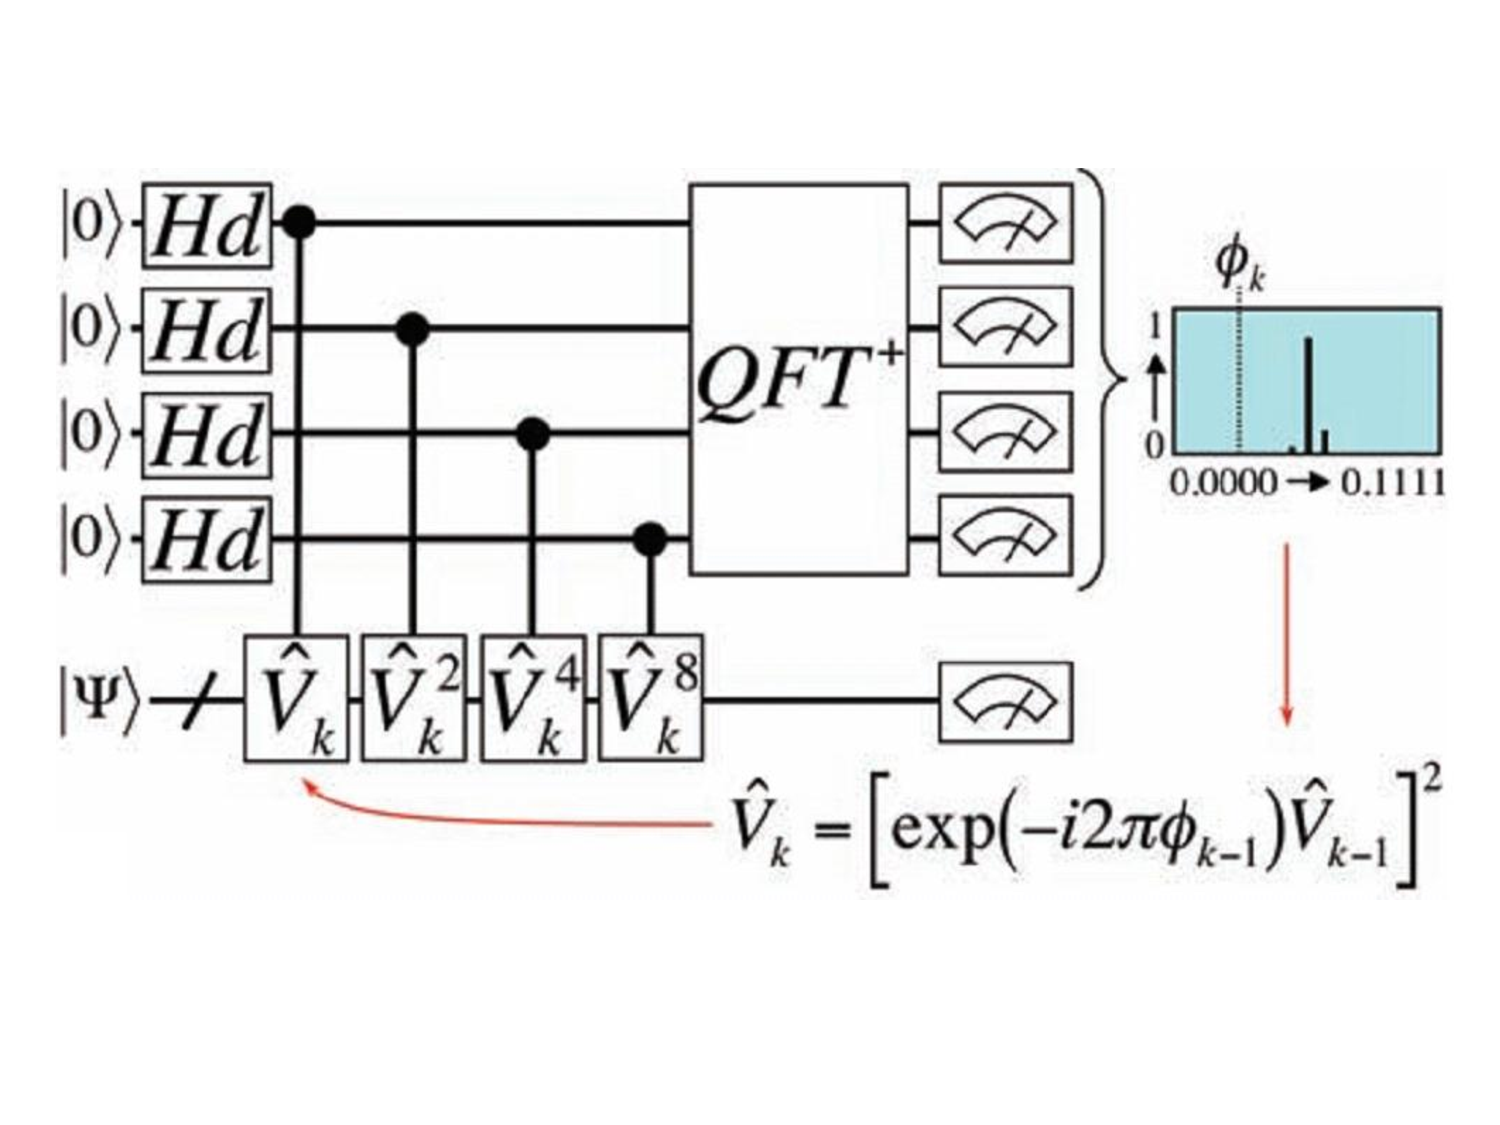
\includegraphics[width= 0.8\columnwidth]{figures/moleculenet.pdf}
              \caption{递归PEA的量子线路图。$k$次迭代是为了得到相位$\phi$的$k$比特精度,从而可以计算分子能级。$QFT^{\dagger}$表示的量子反傅里叶变换,$H_d$为Hadamard操作。取自[Science 309, 1704 (2005)\cite{Alan_first}]. }\label{moleculenet}
            \end{center}
 \end{figure}

其次是受控演化。受控演化的目的就是为了执行PEA算法,以在辅助qubit上产生一个相移,而该相移反映了基态能级的信息。
简略来讲,当我们在基态$\left\vert \psi \right\rangle$上施加幺正操作$U=e^{-iH\tau}$后,指数项上将产生一个相位因子
\begin{equation}
U \left\vert \psi \right\rangle =
e^{-iH\tau}\left\vert \psi \right\rangle =
e^{-iE\tau}\left\vert \psi \right\rangle =
e^{i2 \pi \phi}\left\vert \psi \right\rangle,
\end{equation}
其中$E=-2\pi\phi/\tau$就是基态能级的大小。实验上,我们可以通过预估能量$E$的大小来把相位$\phi$局限在0和1之间。如果
辅助qubit的相位可以以很高的精度测量,我们自然可以得到很高精度的本征能量大小。可惜的是,这需要消耗大量的qubit。

为了克服这个困难,Aspuru等人提出了修改的PEA来减少qubit的所需数目,见图\ref{moleculenet}。该线路图的主要思路是递归,即利用公式
\begin{equation}
V_{k+1}=[e^{-i2 \pi \phi_k}V_k]^2
\end{equation}
重复任意$n$-qubit的PEA过程。这里$\phi_k$是在第$k$次迭代时相位$\phi$的下界。整个迭代过程的初始条件为
\begin{equation}
V_{0}=U=e^{-iH\tau}.
\end{equation}
在递归的PEA中。每一步可以得到$\phi$的一个比特的精度,只要把整个PEA重复很多次我们就可以得到足够大的精度。换句话说,不论
qubit的数目$n$多小(甚至只有1个qubit),只要不断地进行PEA的迭代我们都可以得到很精确的结果。

\begin{figure}[htbp]
            \begin{center}
              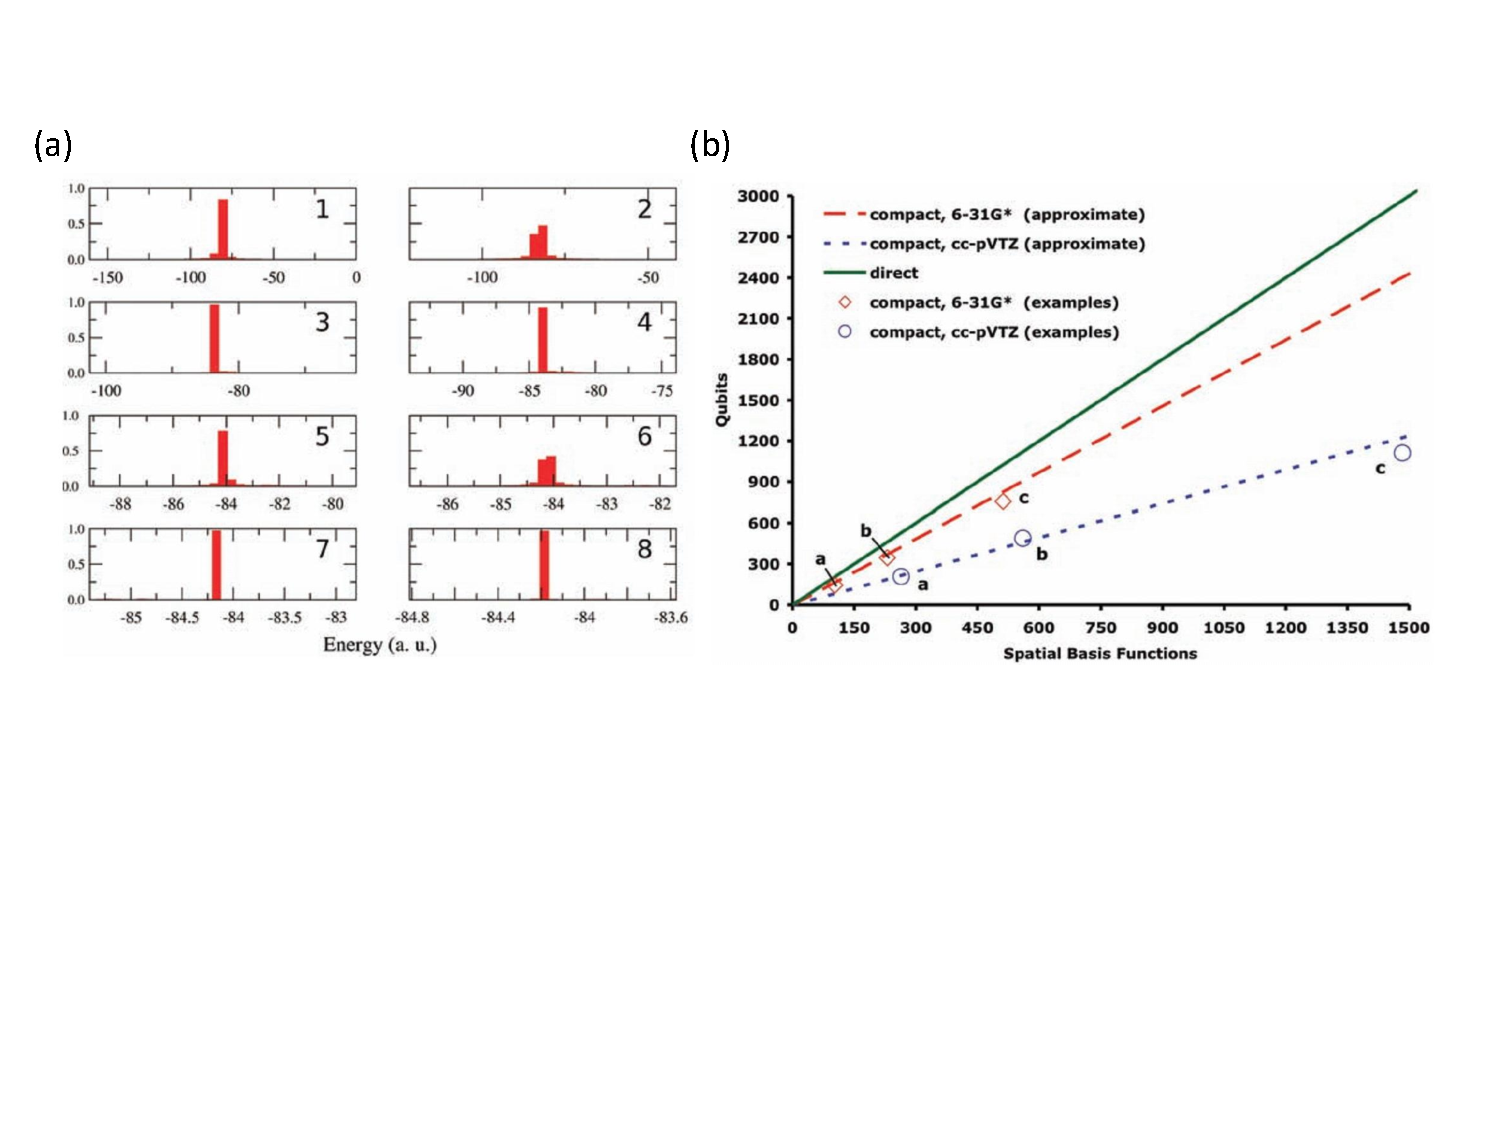
\includegraphics[width= 0.8\columnwidth]{figures/moleculesim.pdf}
              \caption{(a) 模拟水分子基态能级的结果。这里一共迭代了8次,得到了$\phi$的八比特精度。(b) qubit数目的要求随基组增大的变化趋势图。不同的基组函数的选取带来的
              qubit的消耗也是不同的。
              取自[Science 309, 1704 (2005)\cite{Alan_first}]. }\label{moleculesim}
            \end{center}
 \end{figure}

既然基态能级的信息已经被编码到了辅助qubit的相位上,我们可以通过直接测量该相位来得到基态能级的大小。如果施加4 qubit的量子反傅里叶变换来进行相位测量,我们每次迭代就可以
以15/16的成功概率得到正确的一比特精度。

和其他的量子计算和量子模拟任务类似,在量子化学的模拟中,理论依然是超前实验很多的。当前的实验技术并不能支持模拟大分子,但演示性的实验还是可行的。
作为量子模拟通往量子化学的第一步,也是关键的一步,最简单也是最重要的模拟图像就是氢分子的基态能级了。本领域最早的两个实验都选择了这个示例,分别用了线性光学系统\cite{optics_static}和NMR系统\cite{static}。下面的两节我们将回顾这两个实验。

\subsection{线性光学体系模拟氢分子能级}

在2010年,Lanyon等人利用线性光学体系模拟了氢分子基态能级\cite{optics_static}。他们选择的是最简单的STO-3G基组函数进行展开,
最终经过20次迭代,达到了20比特的精度。

\begin{figure}[htbp]
            \begin{center}
              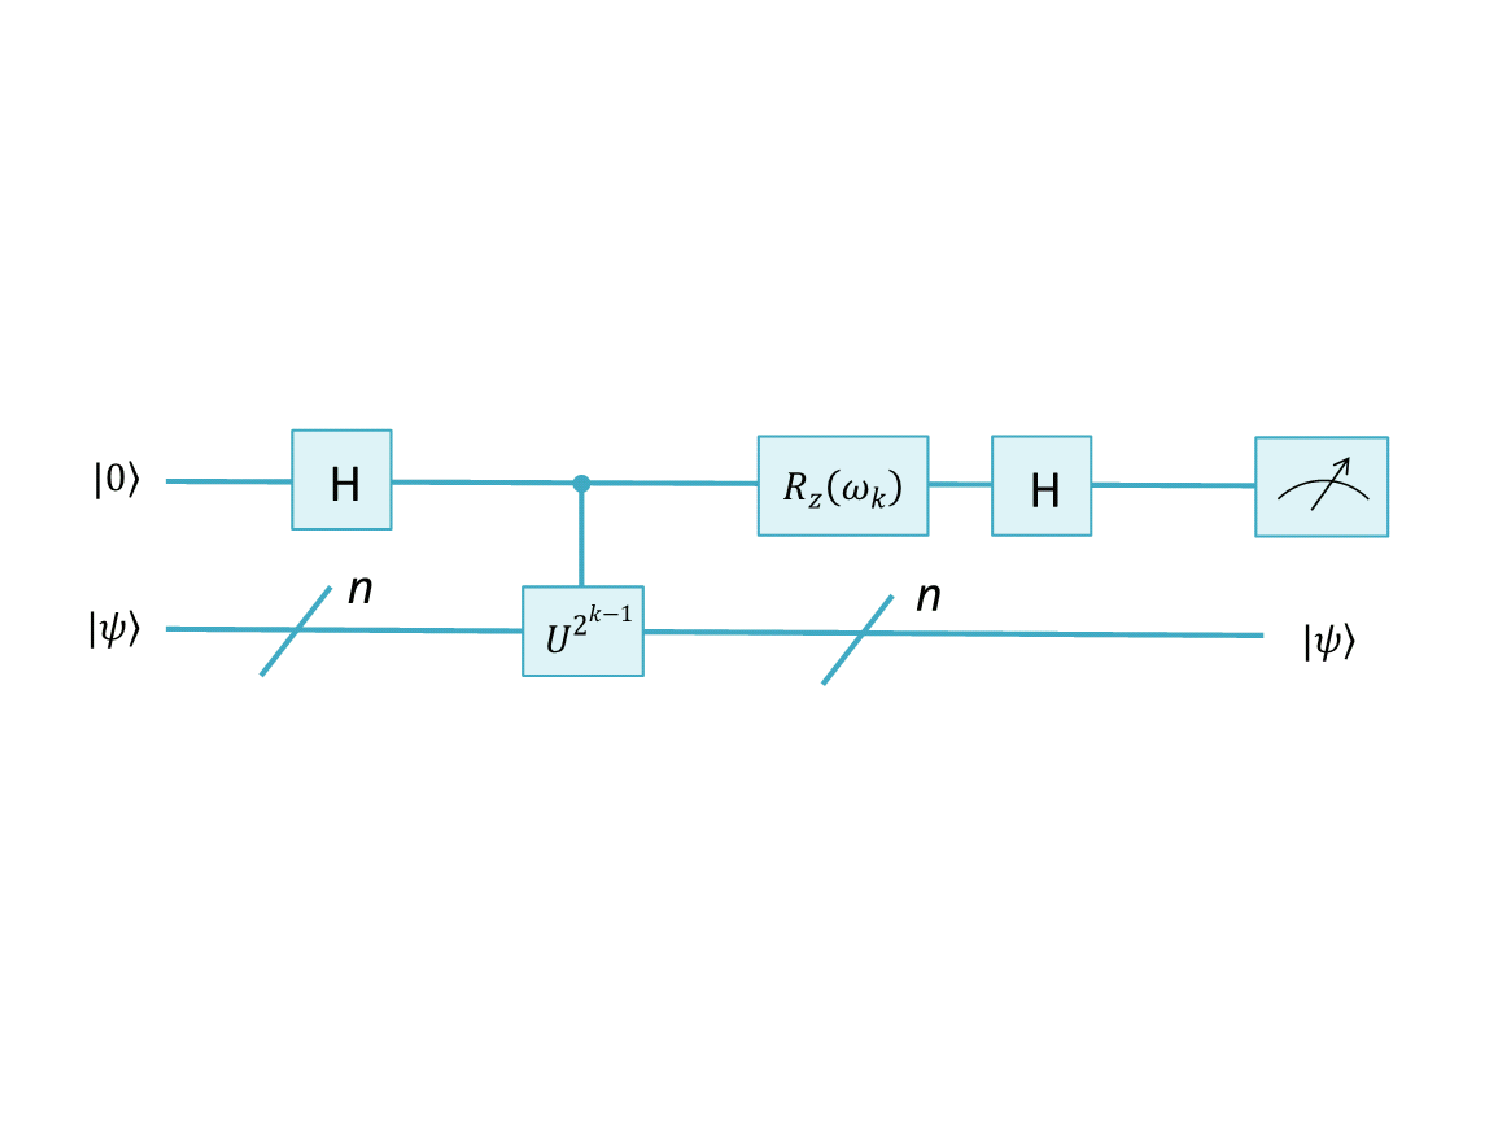
\includegraphics[width= 0.8\columnwidth]{figures/simhydro.pdf}
              \caption{线性光学体系模拟氢分子能级实验中的网络图,其中包含了迭代PEA的过程。
               }\label{simhydro}
            \end{center}
 \end{figure}

在线性光学系统中,qubit的信息被编码到单光子的极化或路径上\cite{hydro1}。比如本实验中,量子态$\left\vert 0 \right\rangle$ and
$\left\vert 1 \right\rangle$和$\left\vert 1 \right\rangle$ and
$\left\vert 1 \right\rangle$分别利用光子的水平及竖直极化$\left\vert H \right\rangle$和$\left\vert V \right\rangle$表示。线性光学实验中,单比特旋转操作是通过
双折射波片实现,而两比特门则是组合了相移器,分束器以及投影测量完成,本实验就是如此。

由于氢分子的哈密顿量是用最简单的STO-3G展开及对角化,所以实验上只需要一个qubit来表征系统波函数,另一个比特就可以用来存储相位信息。
在本实验中,一共用到了两个qubit进行模拟,一个用作系统,另一个用作辅助读出相位信息。而在初态制备阶段,该实验上直接就把系统制备到了氢分子的基态上,而基态形式的计算是借助经典计算机完成。
至于核心步骤迭代PEA则是在线性光学元件上完成的,参见图
\ref{opticnet}。对于每次迭代,实验上将得到一比特的精度,而在整个PEA重复了20次后,最后得到的比特精度为20位(图\ref{simhydro})。最终实验得到的基态能量为
-535.58 $\pm$ 0.03 kJ mol$^{-1}$,这个经典计算机得到的结果是一致的。

\begin{figure}[htbp]
            \begin{center}
              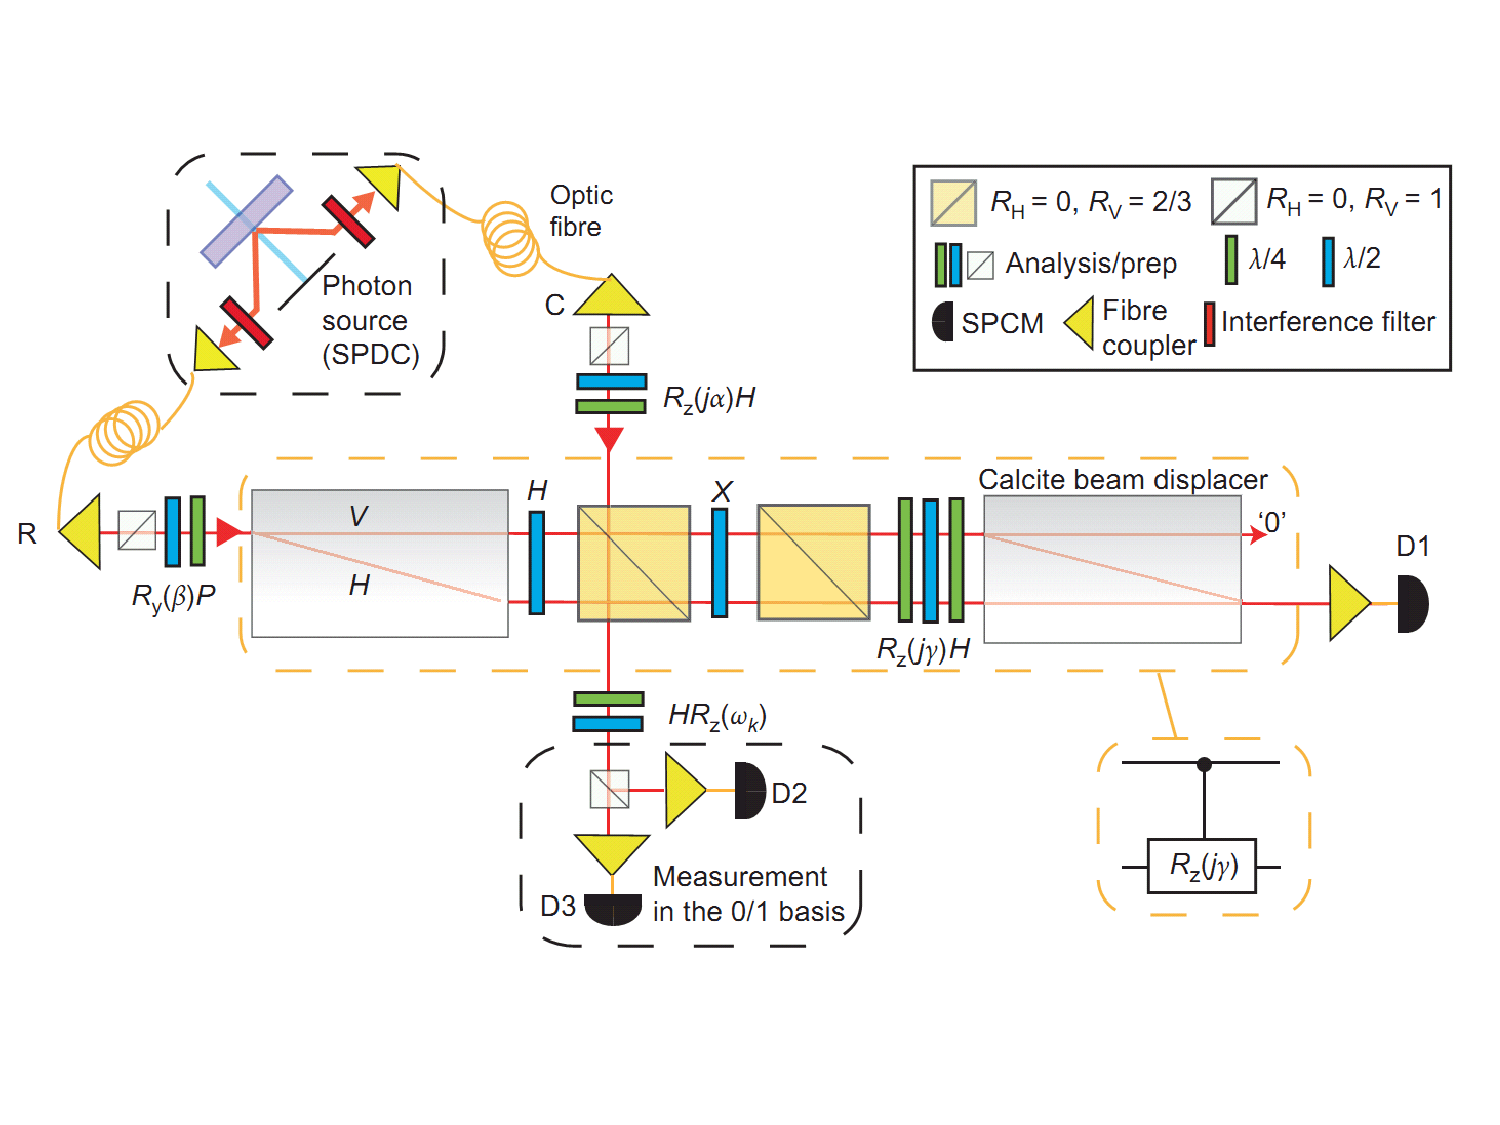
\includegraphics[width= 0.8\columnwidth]{figures/opticnet.pdf}
              \caption{2 qubit PEA的线性光学实现。
              取自[Nat. Chem. 2, 106 (2010)\cite{optics_static}]. }\label{opticnet}
            \end{center}
 \end{figure}
本实验最大的问题是,虽然核心的迭代PEA是在线性光学系统上完成的,但其他的步骤,包括初态制备等等都是利用经典计算机完成的。
因此,很多专家也将该实验描述为"世界上最贵的实现$2\times2$矩阵对角化的实验",因为这些光学器件的价格确实十分昂贵。
尽管如此,该实验作为量子化学模拟的早期尝试,仍然有一定的意义。而在文章的最后,作者还详细讨论了实验上的可扩展性。

\subsection{NMR体系模拟氢分子能级}

几乎和线性光学的实验同时,我们也利用NMR系统模拟了氢分子的基态能级\cite{static}。在NMR实验中,我们选择的也是
广泛应用的STO-3G基组函数,而利用的样品则是$^{13}$C标记的2 qubit氯仿样品。在样品中, $^{13}$C用作系统qubit而$^{1}$H
用作辅助qubit。我们在实验上的基态制备是利用的绝热态制备方法(adiabatic state preparation, ASP)。首先我们在理论上模拟了不同核间距离时
ASP的效率,见图\ref{nmrhydroasp},并最终选择了$r=1.4$ a.u. 作为实验上的数据点。迭代PEA过程我们一共用了15次,每一次得到3比特的精度,也就是
总共会得到45比特的精度。相位读出我们选择了利用NMR干涉仪\cite{hydro2,hydro3,hydro4},来得到辅助qubit上的相位信息。
最终我们实验上得到的基态非常精确,仅仅在45个比特的最后一位上和理论上有差别。下面我们将详细介绍整个实验。

\begin{figure}[htbp]
            \begin{center}
              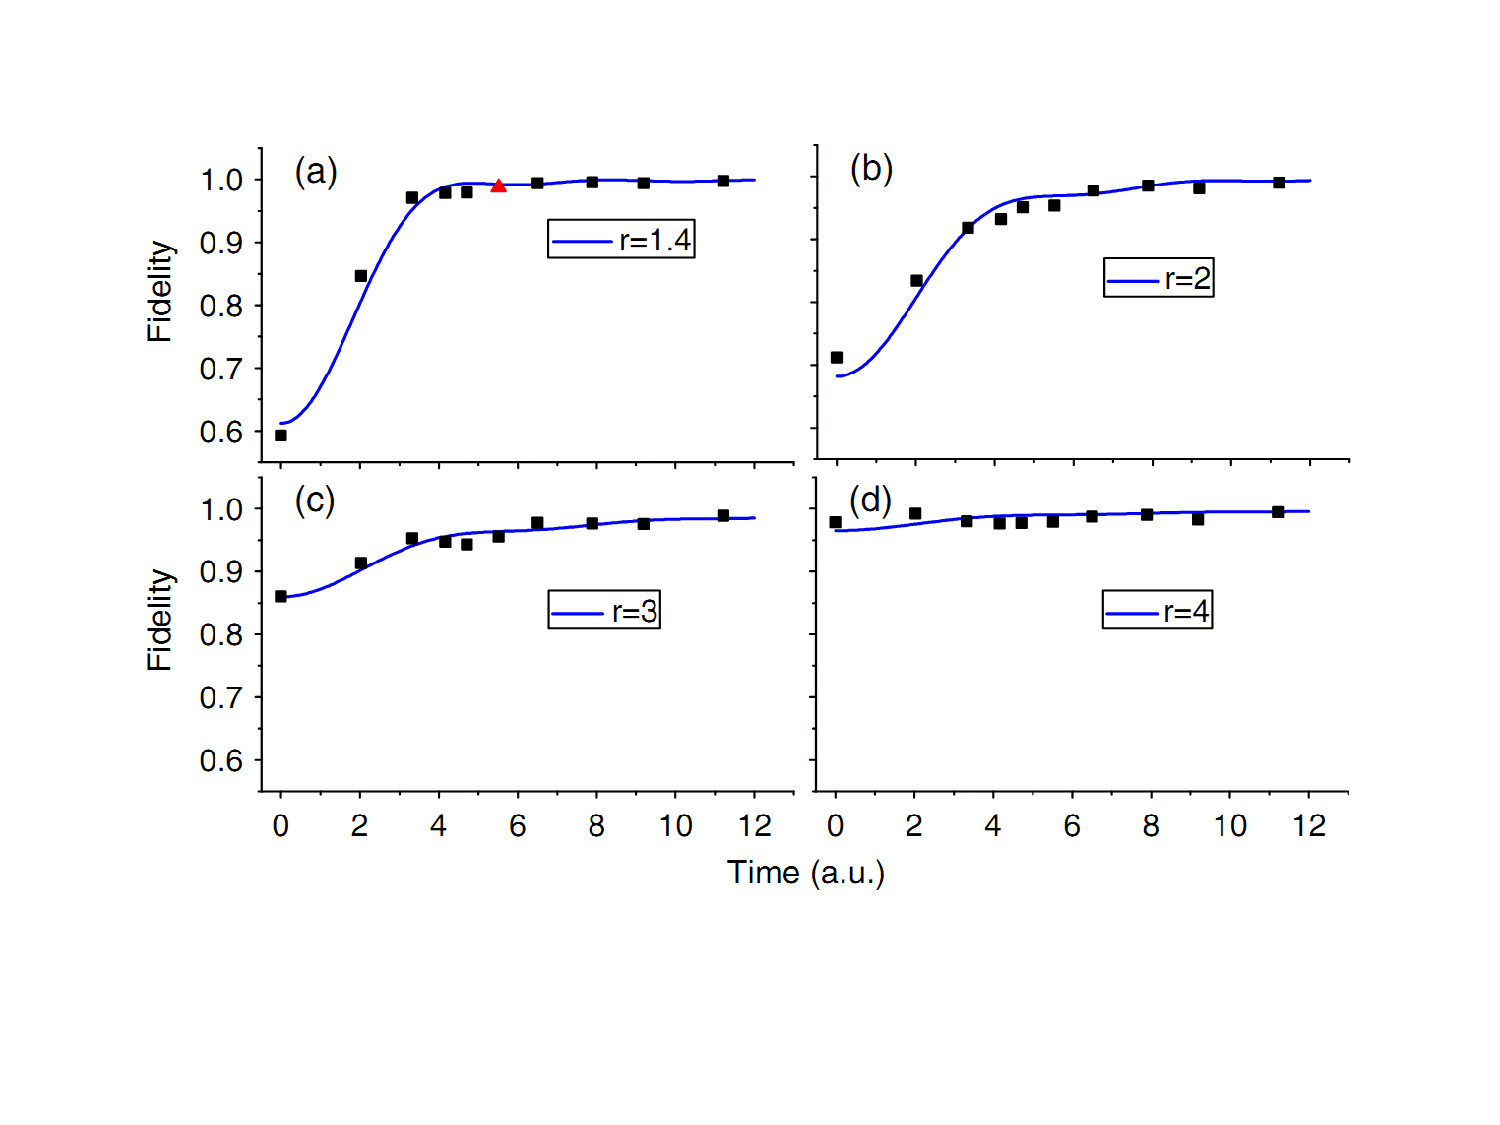
\includegraphics[width= 0.8\columnwidth]{figures/nmrhydroasp.pdf}
              \caption{对于不同的核间距离,我们测试了ASP的保真度随时间变化的函数。依据绝热定理,随着演化时间的增加ASP的保真度
              是趋向于1的。方块为数值模拟的结果,而三角就是实验上ASP选择的点。模拟上绝热过程我们分了100步,而在实验上用了8步。}\label{nmrhydroasp}
            \end{center}
 \end{figure}
理论上,在引入Born-Oppenheimer近似后,氢分子的哈密顿量形式可以写为
 \begin{eqnarray}
\mathcal{H}=&&\sum\limits_{i=1}^2 (T_i+\sum\limits_{j=1}^2V_{ij})+\sum\limits_{i,j=1,i>j}^2O_{ij},
\end{eqnarray}
其中$T_i$是第$i$个电子的动能,$V_{ij}$是第$i$个电子与第$j$个原子核之间的库仑势能,$O_{ij}$则是第$i$个电子与第$j$个电子
之间的库仑势能。在考虑了单态对称性和空间对称性后,STO-3G中展开的氢分子哈密顿量形式可以简化为
\begin{eqnarray}
        H&=&
        \begin{pmatrix}
            \langle\Psi_0|H|\Psi_0\rangle & \langle\Psi_{1\bar{1}}^{2\bar{2}}|H||\Psi_{1\bar{1}}^{2\bar{2}}\rangle\\
            \langle\Psi_{1\bar{1}}^{2\bar{2}}|H|\Psi_0\rangle & \langle\Psi_{1\bar{1}}^{2\bar{2}}|H|\Psi_{1\bar{1}}^{2\bar{2}}\rangle
            \end{pmatrix}\nonumber\\
        &=& \begin{pmatrix}
            -1.8310 & 0.1813\\
            0.1813 & -0.2537
            \end{pmatrix},
\end{eqnarray}
该哈密顿量的基态本征值为-1.85157092935119 a.u.。这里给出15比特的精度是为了后面方便比较实验和理论的结果。

\begin{figure}[htbp]
            \begin{center}
              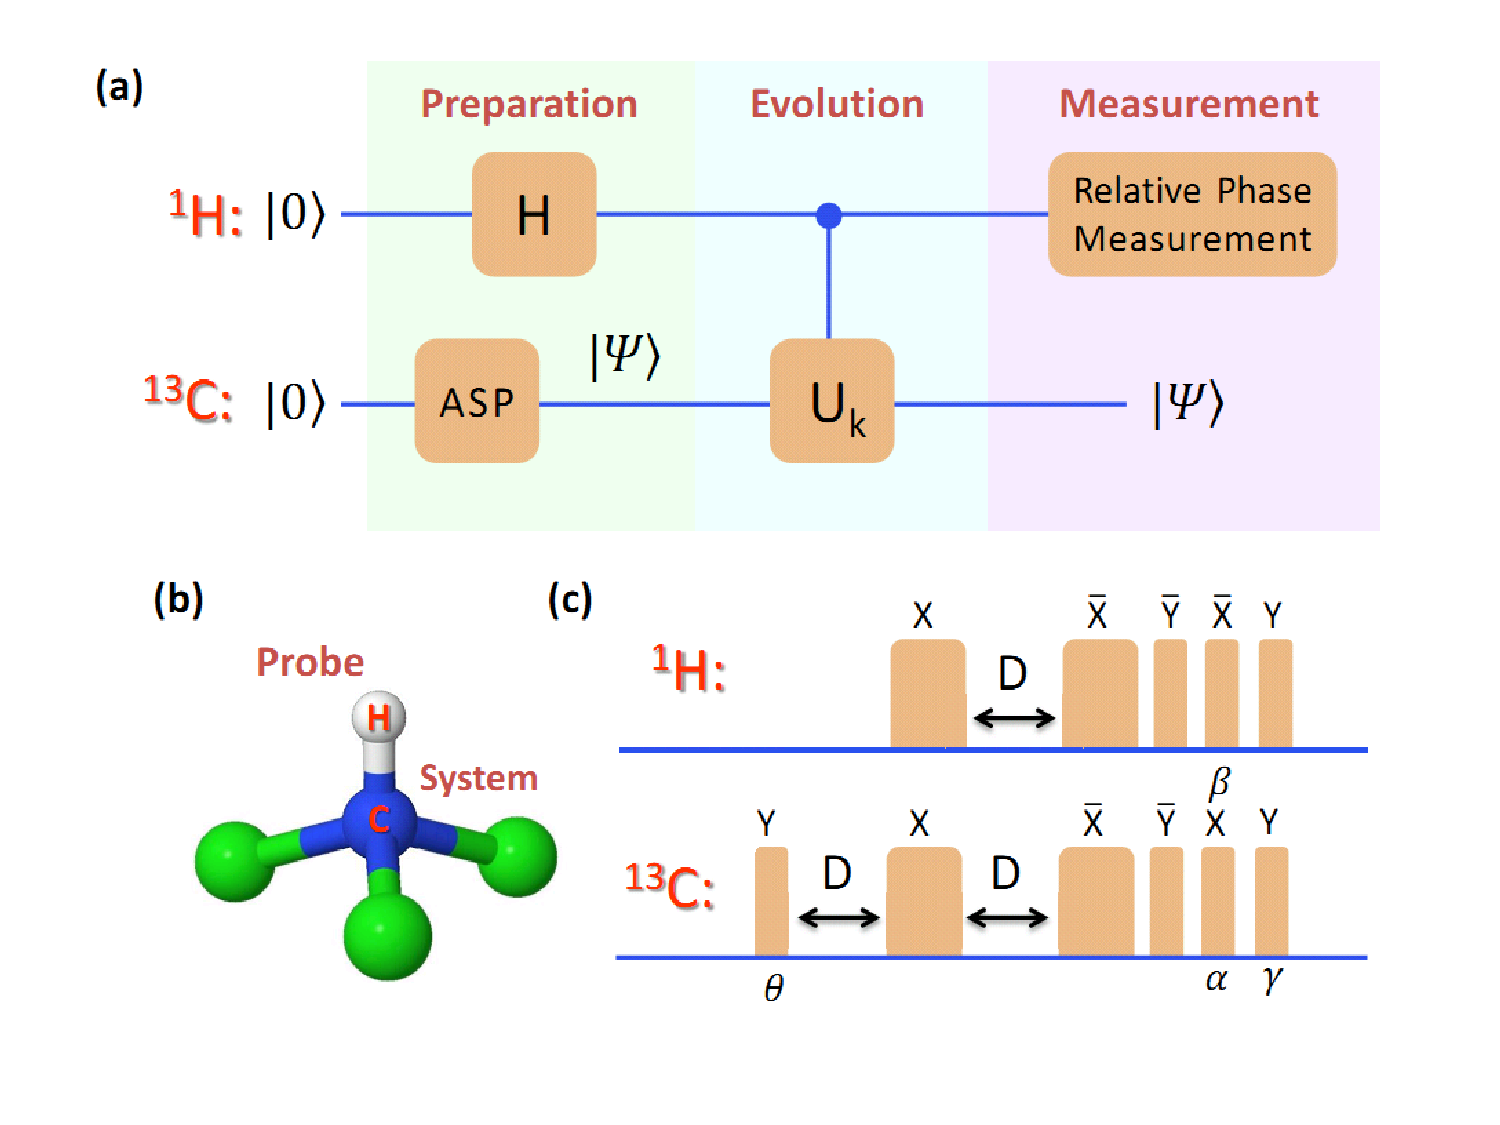
\includegraphics[width= 0.8\columnwidth]{figures/nmrhydronet.pdf}
              \caption{(a) NMR模拟氢分子能级的网络图。(b) 实验上用到的2 qubit量子寄存器CHCl$_3$的分子结构图。(c) 执行控制$U_k$操作的脉冲序列,其中
              对第$k$次迭代来说,$\theta =$ arctan$(\frac{2H(1,2)}{H(1,1)-H(2,2)})=0.226$, $\gamma = \frac{\pi}{2}-\theta=1.3458$, $\beta = \beta_k^0-\phi_{k-1}'$,$\alpha = \frac{8^{k-1}\tau}{2}\sqrt{4H(1,2)^2+(H(1,1)-H(2,2))^2}$,$D=\frac{\alpha}{\pi J_{wa}}$。实验上总计进行了15次迭代。}\label{nmrhydronet}
            \end{center}
 \end{figure}

实验上我们选择利用$^{13}$C标记的2 qubit氯仿中的$^{13}$C用作系统qubit,而$^{1}$H
用作辅助qubit。该分子的结构见图\ref{nmrhydronet}(b),其中两个qubit已经被标记出来。
该系统的内部哈密顿量为
\begin{eqnarray}
\mathcal{H}_{int}=\frac{\omega_{H}}{2}\sigma_{z}^H+\frac{\omega_{C}}{2}\sigma_{z}^{C}+\frac{\pi
J_{CH}}{2}\sigma_{z}^{H}\sigma_{z}^{C},
\end{eqnarray}
其中$\omega_{H}/2\pi$和$\omega_{C}/2\pi$分别是Larmor频率,$J_{CH}$是$J$耦合常数。该样品中$J_{CH}=214.6Hz$。

整个实验过程被分为三个部分:

$\bullet$ 绝热态制备,即把系统qubit $^{13}$C制备到哈密顿量的基态上去。

$\bullet$ 受控哈密顿量演化,以在辅助qubit上产生一个相对相位。

$\bullet$ 测量辅助qubit上的相位,并计算得到能量信息。

(a) \emph{初态制备}

首先我们依然要从热平衡态出发制备PPS
\begin{equation}
\rho_{00} =\frac{1 -
\epsilon}{4} \mathbf{I}+ \epsilon|00\rangle \langle 00|,
\end{equation}
其中 $\mathbf{I}$是$4 \times 4$的单位阵而$\epsilon \approx
10^{-5}$是极化度。然后,我们利用ASP把系统qubit制备到哈密顿量的基态$|\Psi\rangle$上,并同时把辅助qubit制备到
$|+\rangle=\frac{1}{\sqrt{2}}(|0\rangle+|1\rangle)$ 上。

在ASP过程中,我们选择的初始哈密顿量为简单的$H_0 = \sigma _x$,其基态为$|-\rangle=\frac{1}{\sqrt{2}}(|0\rangle-|1\rangle)$。
从PPS出发,我们可以利用共轭的赝Hadamard操作 $R_{y}^{H}
(-\pi/2)$轻松的制备该基态。ASP中缓慢改变的哈密顿量我们选择线性插值的方式
\begin{equation}
H_{ad}=(1-s)\sigma_x + sH,
\end{equation}
其中$s=\frac{t}{T}$。对于每一步的绝热演化来说,我们利用Trotter公式将其演化展开为
\begin{equation}
U_{m}=e^{-i\frac{\delta t}{2}(1-s_m)\sigma_{x}}e^{-is_mH\delta t}
e^{-i\frac{\delta t}{2}(1-s_m)\sigma_{x} }+O({\delta t}^{3}),
\end{equation}
其中$\delta t = T/(M+1)$ 且 $s_m=m/(M+1)$。我们可以利用一个简单的脉冲序列$R_{-x}^{C}(\theta_{1})-R_{-y}^{C}(\theta_{2})-R_{x}^{C}(\theta_{3})$来直接
实现$U_m$,因此整个演化可以通过不断重复这个序列来达到。至此我们就完成了初态制备。

(b) \emph{时间演化}

在时间演化中,我们用到了迭代过程和NMR干涉仪的概念\cite{hydro2,hydro3,hydro4}。

在理论方案中,为了测量相移必须用到4 qubit的QFT。在我们的NMR实验中,由于用到了和光学中类似的干涉仪概念,
其探测灵敏度及精度都比原始的4 qubit QFT要好。实验上我们得到的相移测量精度可以达到$\pm 5^{\circ}$,因此可以保证实验能计算出氢分子能级的任意精度。
迭代的初始条件为$U_0=U$,而迭代形式是
\begin{equation}
U_{k+1}=[e^{-i2\pi\phi_k'}U_k]^{2^n},
\end{equation}
其中$n$是比特数,而$\phi_k'=max\{\phi_k-\phi_{errbd}, 0\}$。


对于控制旋转门来说,其作用可以表示如下:当控制qubit $^1$H处于 $|0\rangle$时,系统qubit $^{13}$C保持不动;而当
控制qubit $^1$H处于 $|1\rangle$时,系统则进行$U_k$的演化。因此整个算子可以表示为
\begin{equation}
C_{U_k}=|0\rangle\langle 0|\otimes I +|1\rangle\langle 1|\otimes U_k.
\end{equation}
在初态
\begin{equation}
|\psi_{in}\rangle=\frac{1}{\sqrt{2}}(|0\rangle+|1\rangle)|\Psi\rangle
\end{equation}
上施加$U_0=e^{-iH\tau}$后,系统将演化到
\begin{equation}
|\psi_{ifm}\rangle=\frac{1}{\sqrt{2}}(|0\rangle+e^{i2\pi\phi}|1\rangle)|\Psi\rangle.
\end{equation}
利用NMR干涉仪的概念我们就可以读出这个相对相位。这里演化时间的大小选择为
\begin{equation}
\tau = [\pi/\sqrt{(2H(1,2))^2+(H(1,1)-H(2,2))^2}].
\end{equation}
实现$C_{U_k}$的脉冲序列见图\ref{nmrhydronet}(c)。

(c) \emph{相位测量}

\begin{figure}[htbp]
            \begin{center}
              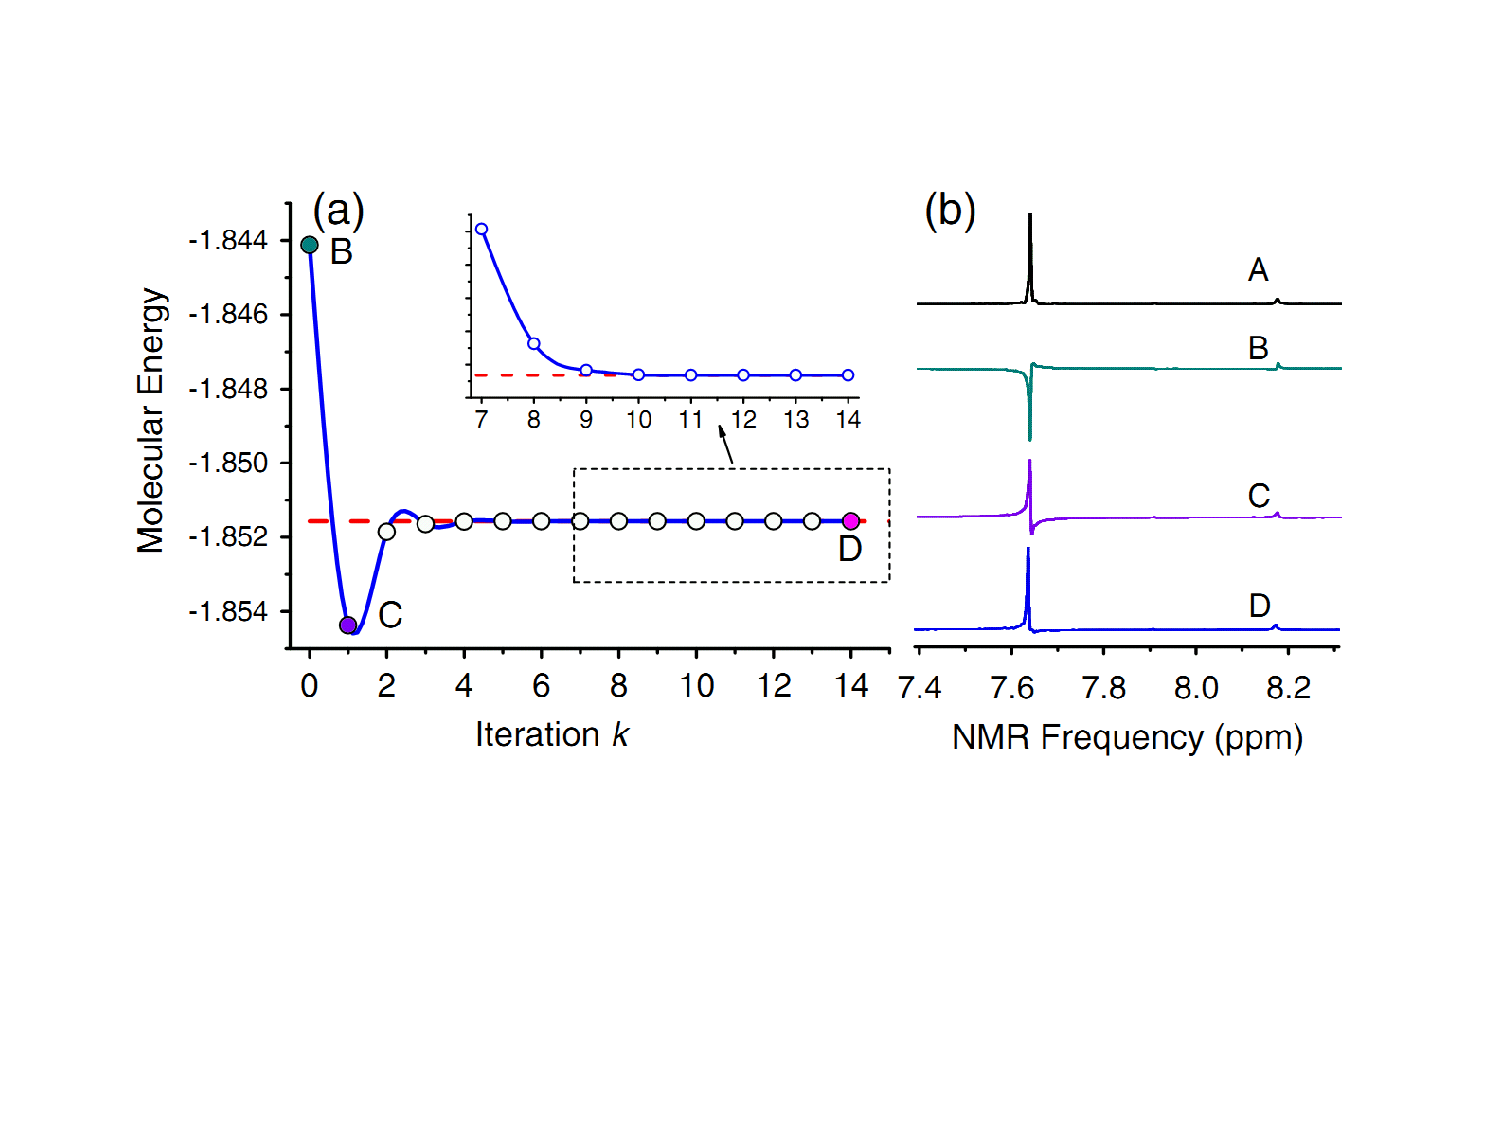
\includegraphics[width= 0.8\columnwidth]{figures/nmrphase.pdf}
              \caption{(a) 15次迭代后测量得到的本征能量大小。圆圈为实验结果,蓝线则是对其拟合的曲线。红色的虚线表示理论值。
              (b) 实验上的$^1$H谱。其中(A)表示的是初态$|\Psi_{in}\rangle$,而(B),(C)和(D)则是在第0,1以及14次迭代后的NMR谱线。从这些谱线上我们可以读出相对相位信息,而这些信息又
              会被用在下一次迭代中。}\label{nmrphase}
            \end{center}
 \end{figure}

在每次迭代之后,我们都要测量相移,并根据迭代形式来调整下一次迭代的算子。NMR中的四极探测可以直接作为
相位探测,如果把初态相位作为基准,那么每次迭代的相对相位都可以直接在NMR谱线上读出(图\ref{nmrphase}(b))。同时,我们把每次迭代后读出的
结果$\phi_k'$用在下一次迭代中。在测量了所有的15个相位后,我们利用迭代的方法重构 $\phi$作为实验结果
\begin{equation}
\phi_i^{result} = \phi_{i+1}^{result}/\phi_{errbd}+\phi_i',
\end{equation}
$\phi_{i+1}^{result}$仅仅是没有物理意义的中间值。最后我们得到的实验结果为-1.851570929351124,而几次中间迭代后的结果参见图\ref{nmrhydroresult}。

\begin{figure}[htbp]
            \begin{center}
              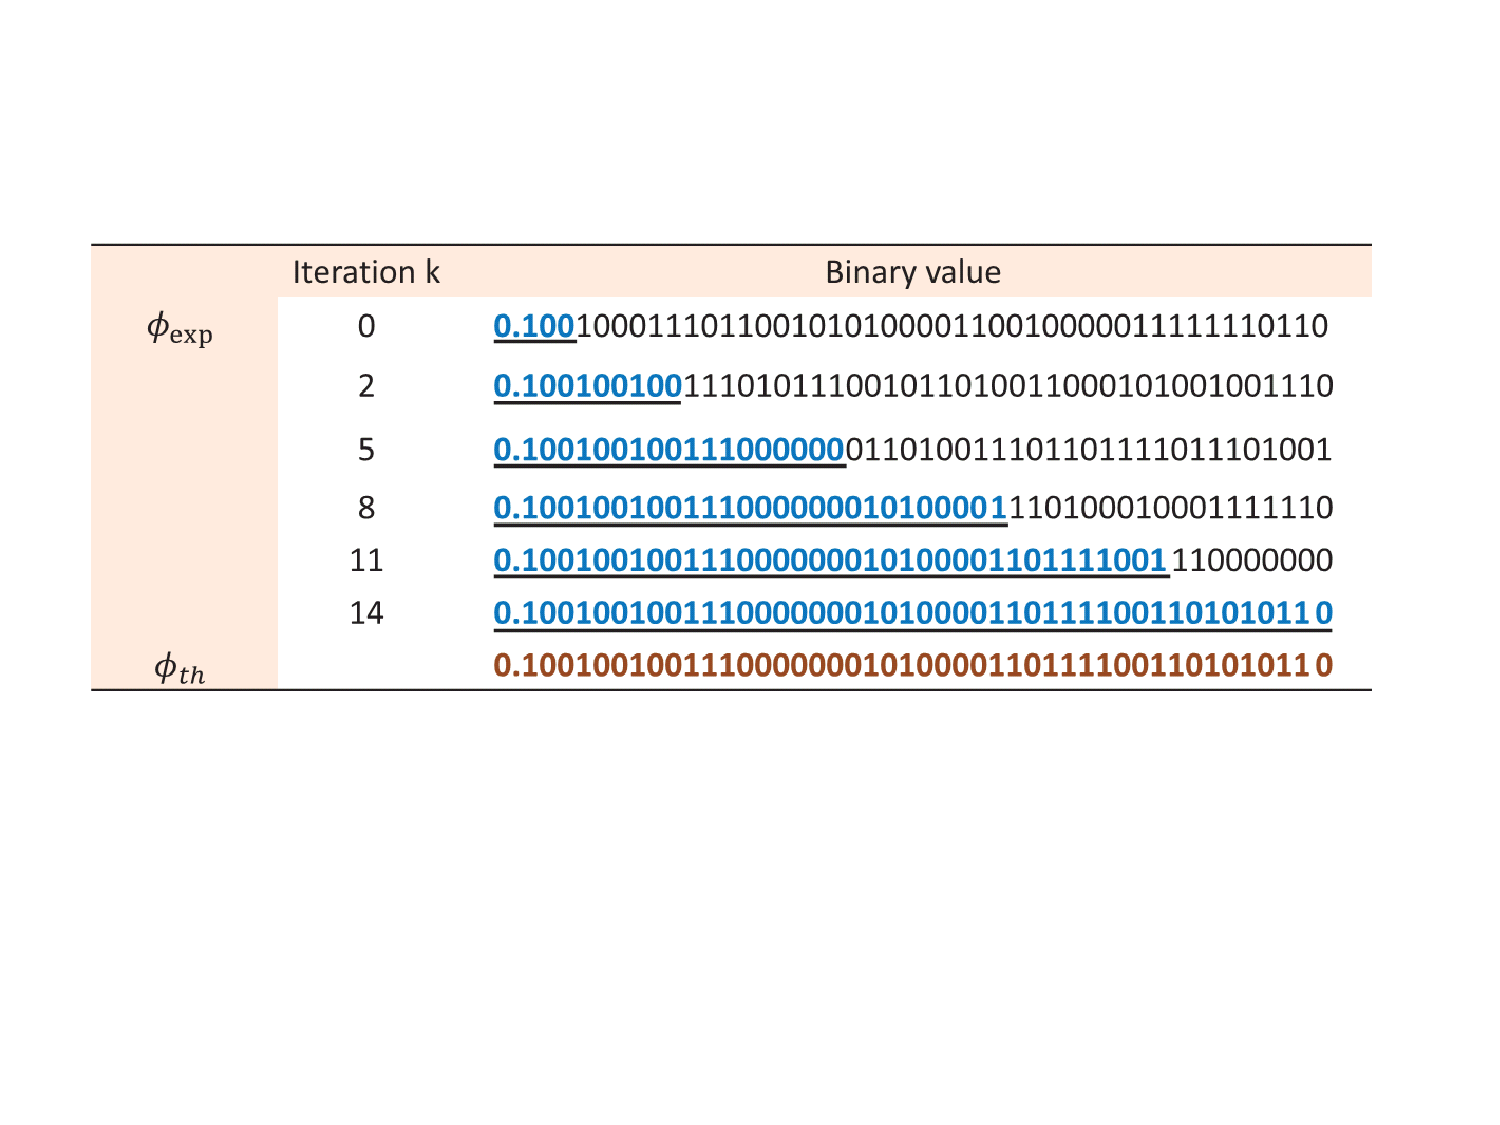
\includegraphics[width= 0.8\columnwidth]{figures/nmrhydroresult.pdf}
              \caption{NMR实验得到的实验值$\phi_{exp}$与理论值$\phi_{th}$的比较。带有下划线的数字为实验得到的结果,每次迭代得到3个比特的精度。
              最终,在15次迭代后,我们得到了45比特的精度。}\label{nmrhydroresult}
            \end{center}
 \end{figure}

 随着要模拟的分子尺度的增大,甚至达到经典计算机无法处理的水平,上面提到的实验方案还适不适合呢?
 我们认为目前的困难主要有两点,只要克服了这两点,就很有希望实现这个目标。第一点是如何有效的拆解分子哈密顿量的演化算子,这在
 Lanyon等人文章的补充材料\cite{optics_static}中进行了详细讨论。他们发现对要模拟的任意分子,逻辑门的数量大概为$N^5$,其中$N$是
 基组函数的数目,也是所需的qubit数目。另外一点是ASP的复杂度问题。现在数值模拟的结果已经达到了128个qubit\cite{hydro5},且为多项式的时间复杂度。
 因此,当必要的硬件及技术困难克服后,量子模拟式可以实现中间尺度的分子的基态能级计算的。

本节的工作已发表在Phys. Rev. Lett. 104, 030502 (2010)\cite{static}上。

\section{动态化学反应的模拟}

“\emph{没有实验室,自然科学就将枯萎。科学家一旦离开实验室,就变成了战场上缴了械的战士。}”

 \hspace{23em} \emph{--巴斯德}

 \subsection{化学反应模拟的理论方案}

 在讨论了静态的分子能级模拟后,接下来我们关注量子化学中的第二个重要任务,也就是化学反应动力学的模拟。
在量子化学中,理解并分析化学反应的机制是一个非常基础的问题。就像之前讨论的,利用经典计算机模拟量子动力学的话随着系统增大需要指数的资源\cite{hydro6}。
而在模拟动力学过程中,由于卷入其中的原子和分子更多,所以它比静态模型的模拟更加复杂。为了解决这个问题,2008年Kassal等人提出了一个指数复杂度的
量子算法\cite{Polynomial_time_algorithm}。该方案利用了一次量子化方法,直接模拟电子与核之间的相互作用演化,而没有采用Born-Oppenheimer近似。当反应涉及到的
原子数目大于4时,采用量子计算的该方案是比经典计算更加有效的。同时,该方案引入了辅助qubit来降低拆解幺正算子的复杂度,当然这涉及了很多的数学计算。辅助qubit
的数目与重构波函数的qubit数目相同,而数值分析也表明该方案是多项式复杂度的,见图\ref{dynamicalcomplex}。

\begin{figure}[htbp]
            \begin{center}
              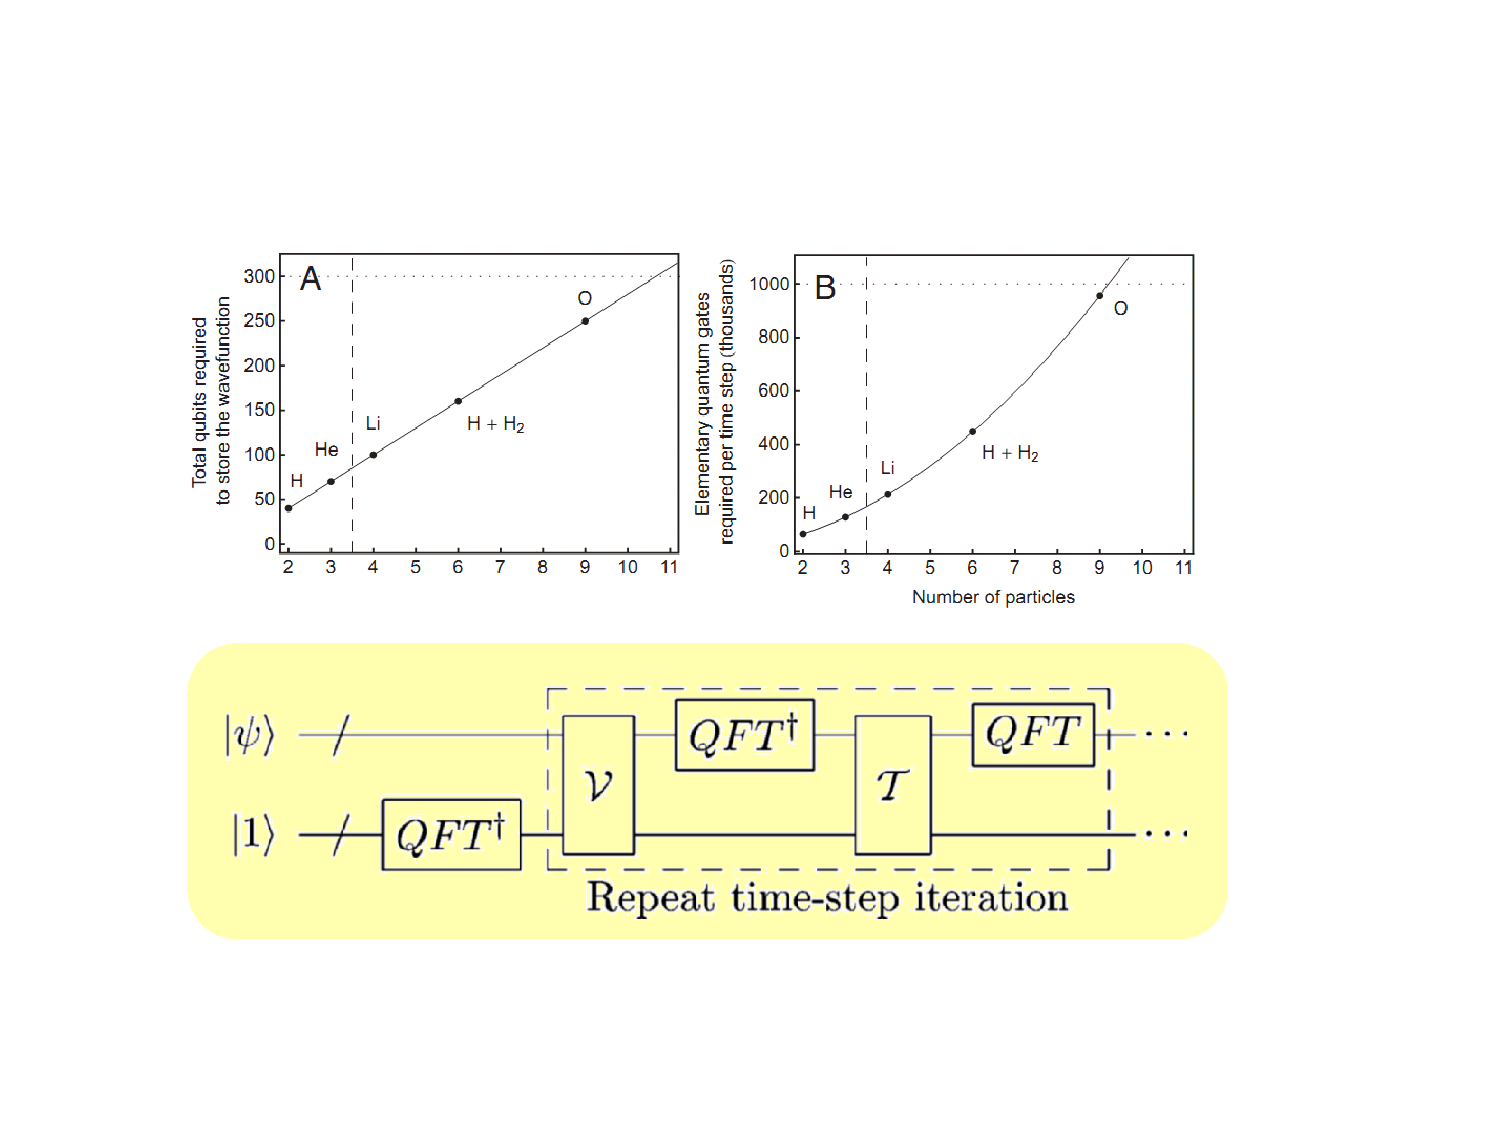
\includegraphics[width= 0.8\columnwidth]{figures/dynamicalcomplex.pdf}
              \caption{随着粒子数的增多,所需的用来存储波函数的qubit数目是线性增加的,而所需的逻辑门数目是多项式增加的。下图为模拟化学反应动力学的网络图。}\label{dynamicalcomplex}
            \end{center}
 \end{figure}

简化起见,我们考虑不含时的哈密顿量,即只依赖于位置的势场。写成公式的话就是
\begin{equation}
\hat{H} = \hat{T}+ \hat{V},
\end{equation}
其中$\hat{T}$ = $\hat{p}^{2}$/2$m$与$\hat{V}$ = $V(\hat{x})$分别是动能和势能算子。一般来说,我们用Trotter公式来分解这个算子
\begin{equation}
 {U}(t+\delta t,t)\approx  e^{-i {V} \delta t/2} e^{-i {E} (t+\delta t/2)  \delta t/2}
 e^{-i {T} \delta t}    e^{-i {E} (t+\delta t/2)           \delta t/2}
 e^{-i {V} \delta t/2} .
\end{equation}
注意到动能算子$e^{ - i \hat{T} \delta t}$与势能算子$e^{ - i \hat{V} \delta t}$分别在动量和位置空间中是对角的,我们可以通过
量子傅里叶变换来实现两者之间的转换,即
\begin{equation}
|\psi (t+\delta t)\rangle  = \hat U(\delta t)|\psi (t)\rangle
  \approx {\rm{QFT}}{e^{-i\hat T\delta t}}
  {\rm{QF}}{{\rm{T}}^{\rm{\dag}}}{e^{-i\hat V\delta t}}|\psi (t)\rangle.
\end{equation}
无论怎么对动能和势能算子转换,都不会影响最后的结果。最后,我们对以上的步骤进行迭代,就可以使得
系统从初态$|\psi(t_0) \rangle$演化到$|\psi(t_f) \rangle$。

除了上述的DQS实现化学反应模拟的方案,AQS也可以用来完成一些化学反应的模拟工作。在半导体量子点\cite{reaction}中,
耦合的量子点可以被认为是"模拟分子",我们可以通过改变一些电学参数来实现模拟不同的反应。而在波导上的冷原子系统\cite{chem3},我们可以通过
极冷原子的运动或者弱相互作用的BEC,来模拟三体的线性化学反应。

 \subsection{NMR实验模拟的异构反应模型}

  \begin{figure}[htbp]
            \begin{center}
              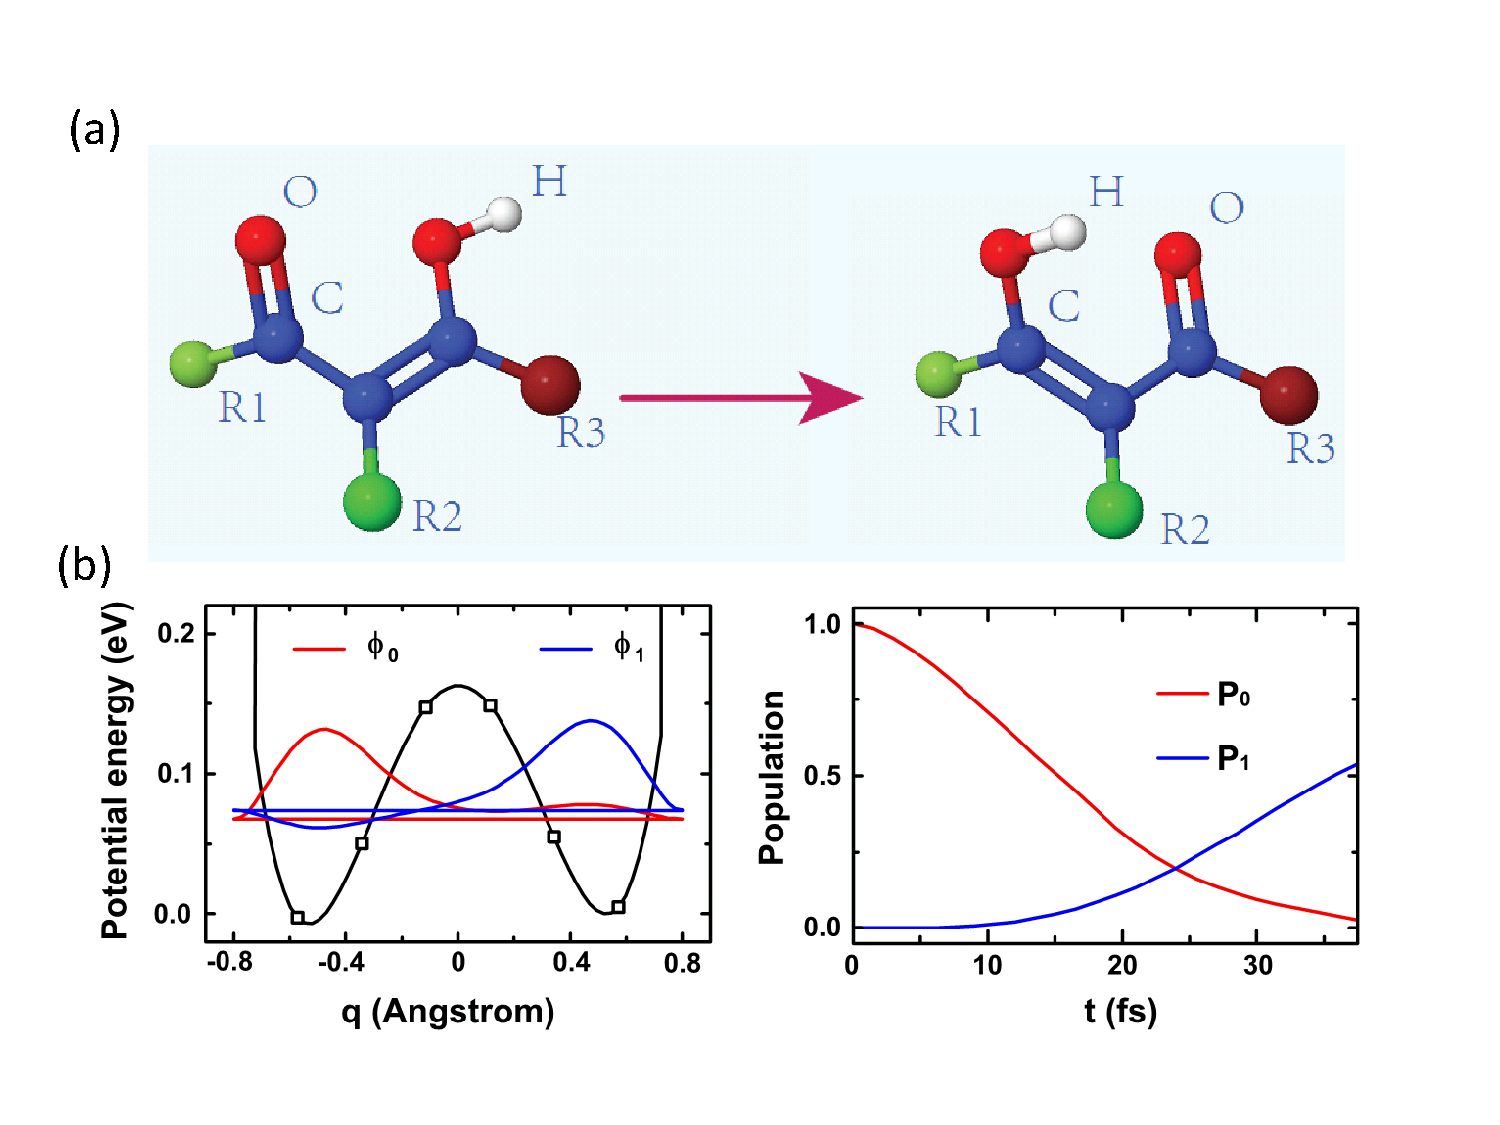
\includegraphics[width= 0.8\columnwidth]{figures/nmrreaction.pdf}
              \caption{(a) 实验上模拟的异构反应。(b) 左边:势能曲线,红线为基态,蓝线为第一激发态。势场中的参数是依照文献\cite{nmrdym1}
              取的,$V^\ddag=0.00625\ E_{\rm h}$,$\Delta=0.000257\ E_{\rm h}$,$q_0=1\ a_0$。右边:基态(反应态,P$_0$)和第一激发态(产物态,P$_1$)随时间的比例分布。}\label{nmrreaction}
            \end{center}
 \end{figure}

 在实验上,我们考虑的是激光诱导的异构反应模型\cite{nmrdym1},见图\ref{nmrreaction}(a)。该反应的好处是一维的,
 而且自由度只有1。从反应图来看,这只是非对称的malonaldehydes上的氢原子转移。在引入外加诱导激光场后,该系统的哈密顿量可以写为
\begin{equation}
  H(t)=  T+  V+  E(t) ,
\end{equation}
其中  $E(t)=- \mu\varepsilon(t)$为外加激光场与分子间的相互作用哈密顿量,$ \mu=e  q$是偶极矩算符,
$\varepsilon(t)$为外加驱动电场,$ {T}={  p}^2/2m$是动能算符,而
\begin{equation}
 {V}=\frac{\Delta}{2q_0}(  q-q_0)+\frac{V^\ddag-\Delta/2}{q_0^4}(  q-q_0)^2(  q+q_0)^2
\end{equation}
是一个双势阱的势场(图\ref{dymmodel}(a))。在势场的表达形式中,$V^\ddag$为势垒高度,$\Delta$表示两个势阱的非对称参数,$\pm q_0$
则给出了势阱最低点所处的位置。

 \begin{figure}[htbp]
            \begin{center}
              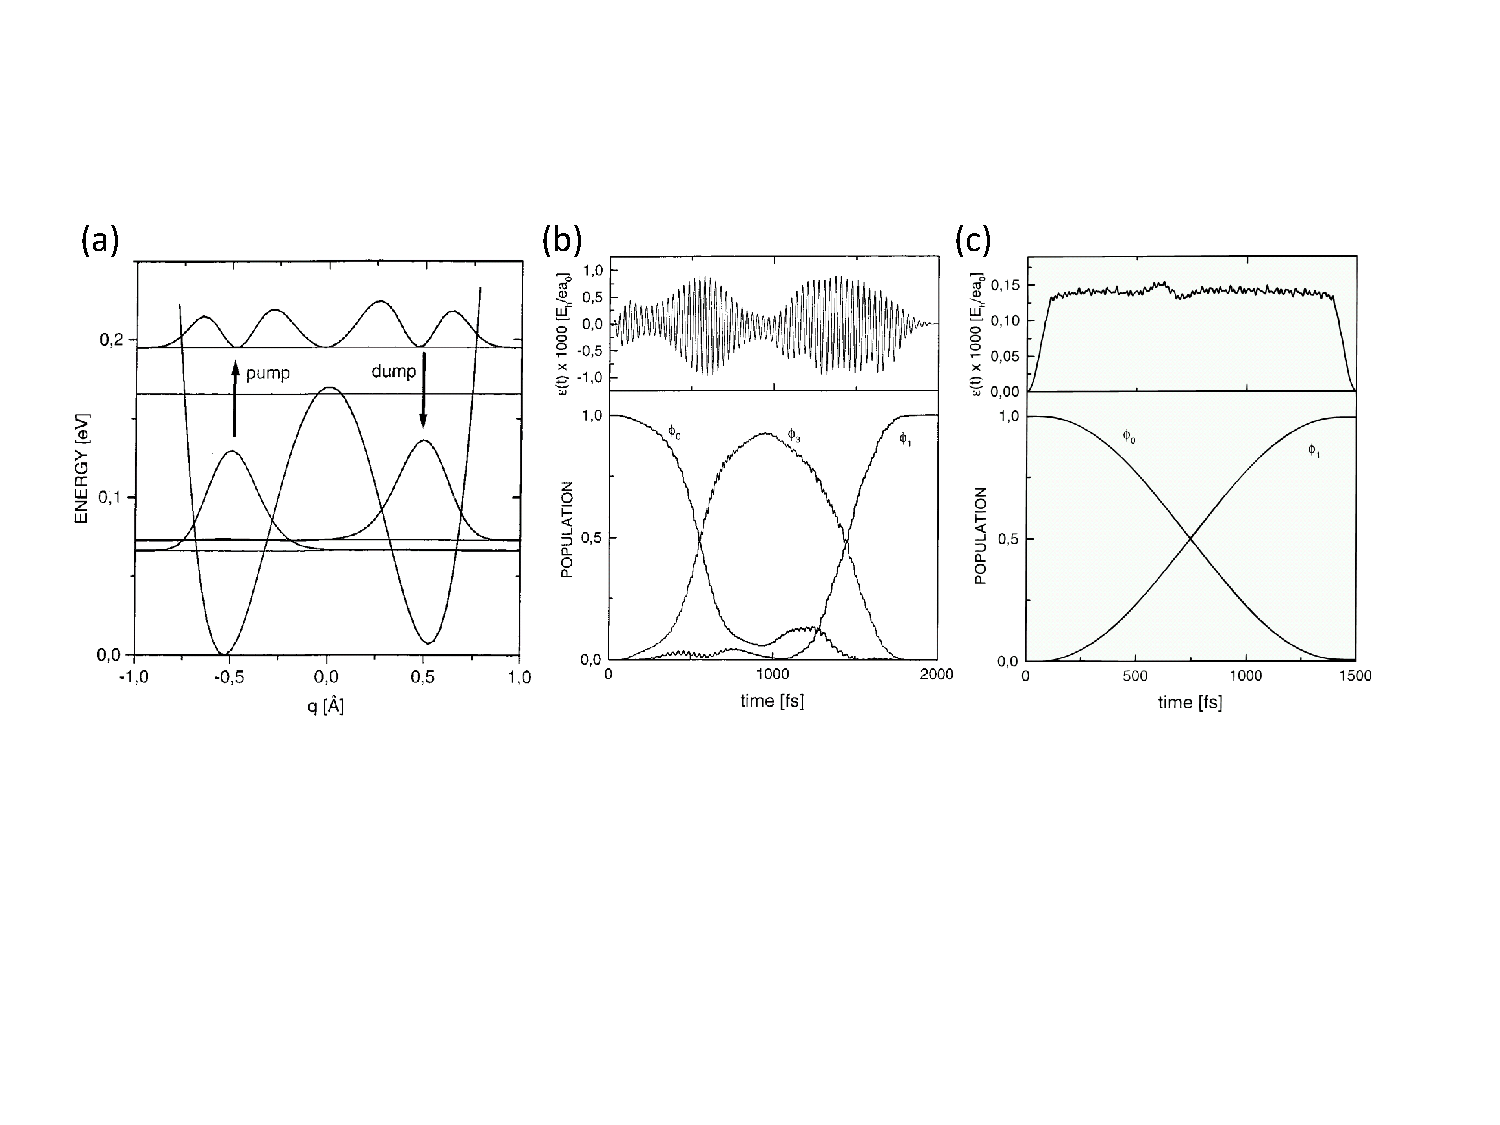
\includegraphics[width= 0.8\columnwidth]{figures/dymmodel.pdf}
              \caption{(a) 异构反应中的双势阱势场形式。利用红外泵浦激光,反应态中的氢原子可以跳过势垒,并转移到产物态上。
              (b) 利用振荡形式的外加激光场产生的反应过程。可以看到,除了反应态$|\phi_0 \rangle$和产物态$|\phi_1 \rangle$,第三激发态也在反应过程中出现了。
              (c) 利用近似梯度的外加激光场,可以看到整个反应中只有反应态$|\phi_0 \rangle$和产物态$|\phi_1 \rangle$,这是因为和传统的"跳过势垒"的方法不同,这里是直接利用量子隧穿效应穿过势垒的,类似于现实生活中的地铁。 }\label{dymmodel}
            \end{center}
 \end{figure}

 首先我们利用Trotter公式给出$t$到 $t+\delta t$时间内的演化算子$ {U}(t+\delta t,t)$
 \begin{equation}
 {U}(t+\delta t,t)\approx  e^{-i {V} \delta t/2} e^{-i {E} (t+\delta t/2)  \delta t/2}
 e^{-i {T} \delta t}    e^{-i {E} (t+\delta t/2)           \delta t/2}
 e^{-i {V} \delta t/2} .
\end{equation}
其中算子$e^{-i {T}\delta t/\hbar}$在动量表象中是对角化的,而其他所有算子在位置空间中也都是对角化的。
如果我们利用QFT,就可以在两个表象之间进行变换。同时,为了给出整个动力学过程的即时状态,我们把反应过程分成了
25个小步,每一步的时间为$\delta t=1.5$fs,因此总的演化时间为$t_f=37.5$fs。对于外加的含时电场,我们选择了一个梯形的形式,类似图\ref{dymmodel}(c),其具体的函数形式为
 \begin{equation}
  \varepsilon(t)=\left\{
    \begin{array}{cc}
       \varepsilon_0\sin^2(\frac{\pi t}     {2s_1})         ;&\qquad   0\leq t\leq s_1\\
       \varepsilon_0                                        ;&\qquad   s_1<t<s_2\\
       \varepsilon_0\sin^2[\frac{\pi(t_f-t)}{2(t_f-s_2)}]   ;&\qquad   s_2\leq t\leq t_f
    \end{array}
  \right.
\end{equation}
在该函数形式中,$s_1=5$fs 且 $s_2=32.5$fs。

在$t=0$时,反应态为哈密顿量$T+V$的基态$\left\vert \phi_{0} \right\rangle$,也就是限制在势场中左边势阱的状态。
产物态则为哈密顿量$T+V$的第一激发态$\left\vert \phi_{1} \right\rangle$,主要限制在右边的势阱中。同时,定义反应系统随时间变化的
波函数为$\left\vert \psi({t}) \right\rangle$。

经过以上分析,我们已经有了系统的哈密顿量,初始的反应态,最后的产物态,以及拆解演化算子的方法,那么下一步就是把
含时波函数$\left\vert \psi({t}) \right\rangle$与算子$T$, $V$, $E(t)$编码到qubit形式。我们利用$N=2^n$个离散的位置基矢来表征这些算子的形式,比如
波函数就可以编码为
\begin{equation}
\left\vert \psi(t) \right\rangle=\sum_{q=0}^{2^n-1}m_q(t)\left\vert q \right\rangle
=m_0(t)\left\vert 0\cdots00 \right\rangle+...+m_{2^n-1}(t)\left\vert 1\cdots11 \right\rangle.
\end{equation}
在实验中,我们用了$n=3$个qubit进行了8个点的离散化过程。编码后的$T$, $V$和$q$为对角矩阵的形式。图\ref{nmrreaction}(b) 给出了8个点离散化的形式,我们发现这个8维的Hilbert空间非常接近于
理论上精确计算的结果(64个离散的点)。同时,两个势阱中概率分布的不平衡性也得到了体现,比如在右边的势阱中测量得到第一激发态的概率为
$80\%$。

\subsection{NMR实验过程}

实验上我们选择的样品为3 qubit Diethyl-fluoromalonate,其中的三个原子核$^{19}$F, $^{13}$C, 和$^1$H
被用作3个qubit。该样品的结构图见图\ref{nmrdymnet}(a),三个qubit被椭圆标记出。该系统的哈密顿量为
\begin{eqnarray}
\mathcal{H}_{int}=&&\sum\limits_{j=1}^3 {2\pi \nu _j } I_z^j  + \sum\limits_{j < k,=1}^3 {2\pi} J_{jk} I_z^j I_z^k,
\end{eqnarray}
其中$\nu_j$是第$j$个自旋的共振频率,$\emph{J}_{jk}$则是第$j$和$k$个自旋的偶极耦合常数。所有的实验都是在室温下Bruker Avance 400 MHz的谱仪上完成的。

 \begin{figure}[htbp]
            \begin{center}
              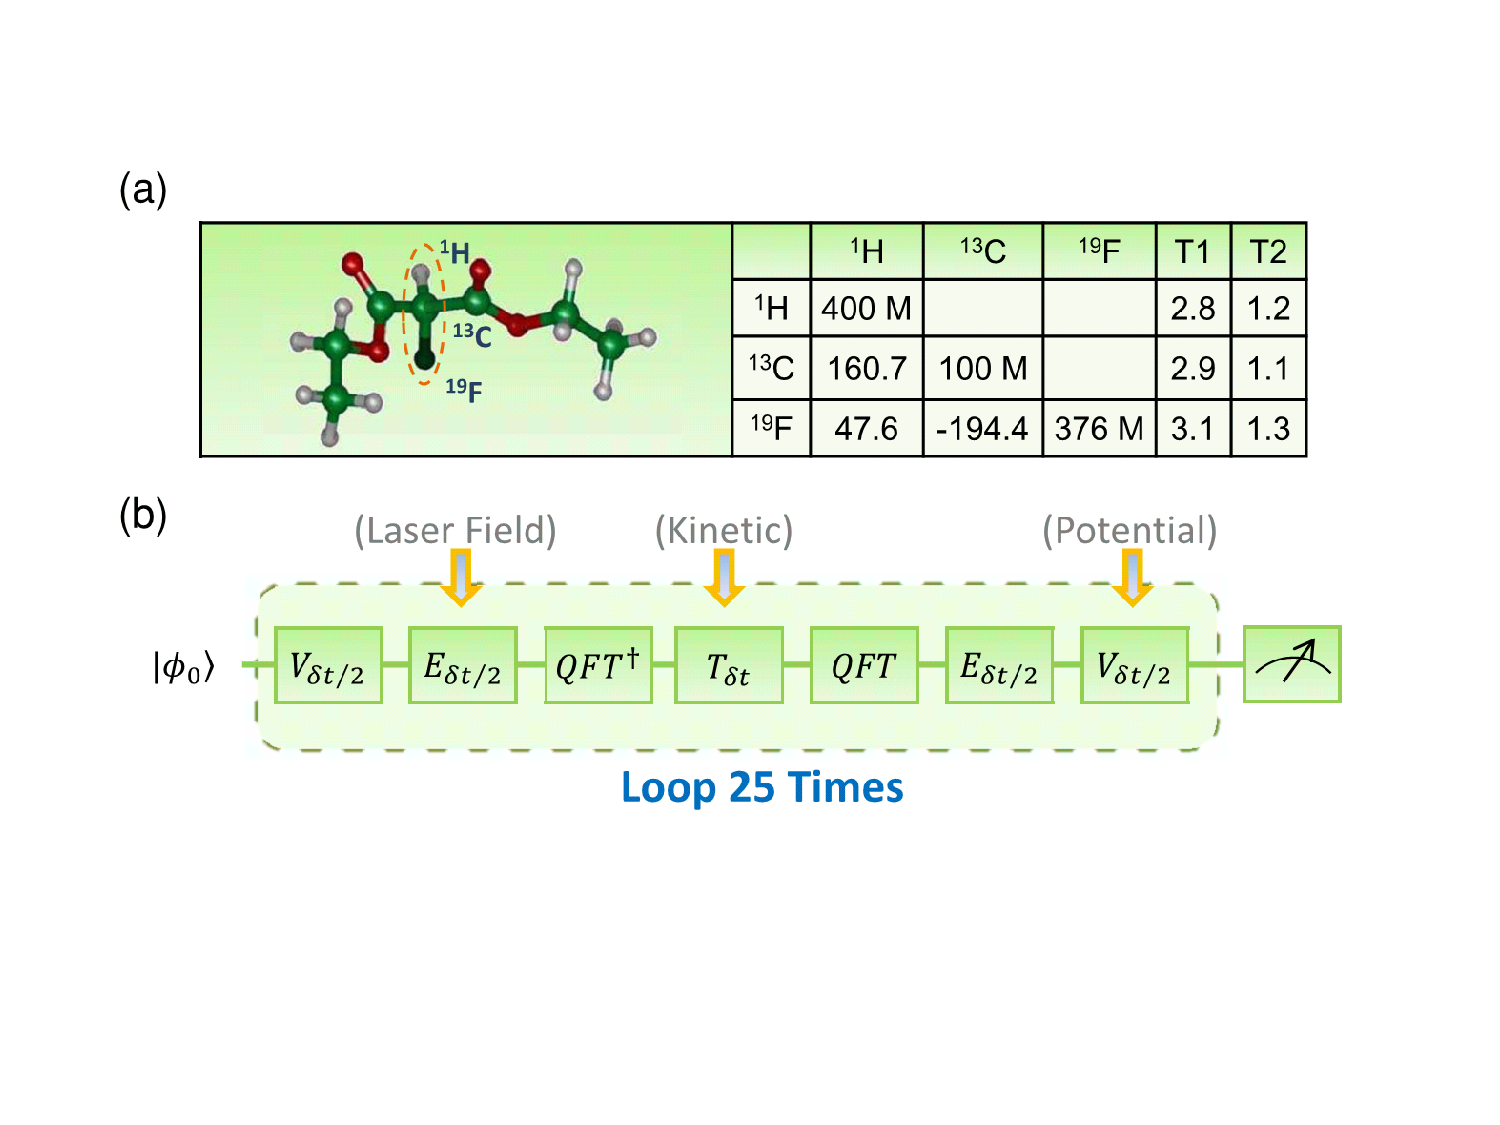
\includegraphics[width= 0.8\columnwidth]{figures/nmrdymnet.pdf}
              \caption{(a) Diethyl-fluoromalonate的分子结构以及系统参数。椭圆标记的$^{19}$F, $^{13}$C, 和$^1$H核自旋被用作3个qubit,而表中则给出了
              3个原子核的Larmor频率,$J$耦合常数以及弛豫时间。(b) 模拟异构动力学反应的逻辑网络图,初态为$\left\vert \phi_{0} \right\rangle$。整个过程被分为了25个循环,每一步的算子
              $T_{\delta t}$, $V_{\delta t}$以及$E_{\delta t/2}$ 都是对角形式的。}\label{nmrdymnet}
            \end{center}
 \end{figure}

 整个实验和大多数的量子计算实验一样,依然分为三个部分:

 $\bullet$ 初态制备。在这个部分我们要制备出哈密顿量$T+V$的基态$\left\vert \phi_{0} \right\rangle$作为反应态。

 $\bullet$ 动力学演化。我们要执行精确的系统演化以模拟连续的化学反应动力学过程。

 $\bullet$ 交叠度测量。对于实验上分的25步,我们要在每一步后测出此时反应态和产物态的比率。在第$j$个循环$t_j\equiv j\delta t$后,我们
 要测量两个交叠度$C(| \psi(t_j) \rangle,| \phi_{0} \rangle)=| \langle\phi_0|\psi(t_j)\rangle |^2$ and $C(| \psi(t_j) \rangle,| \phi_{1} \rangle)=
|\langle\phi_1|\psi(t_j)\rangle |^2$,这也就是即时的反应物和产物的比例。通过这个数值,我们可以绘制出反应物转化为产物的曲线。

 \begin{figure}[htbp]
            \begin{center}
              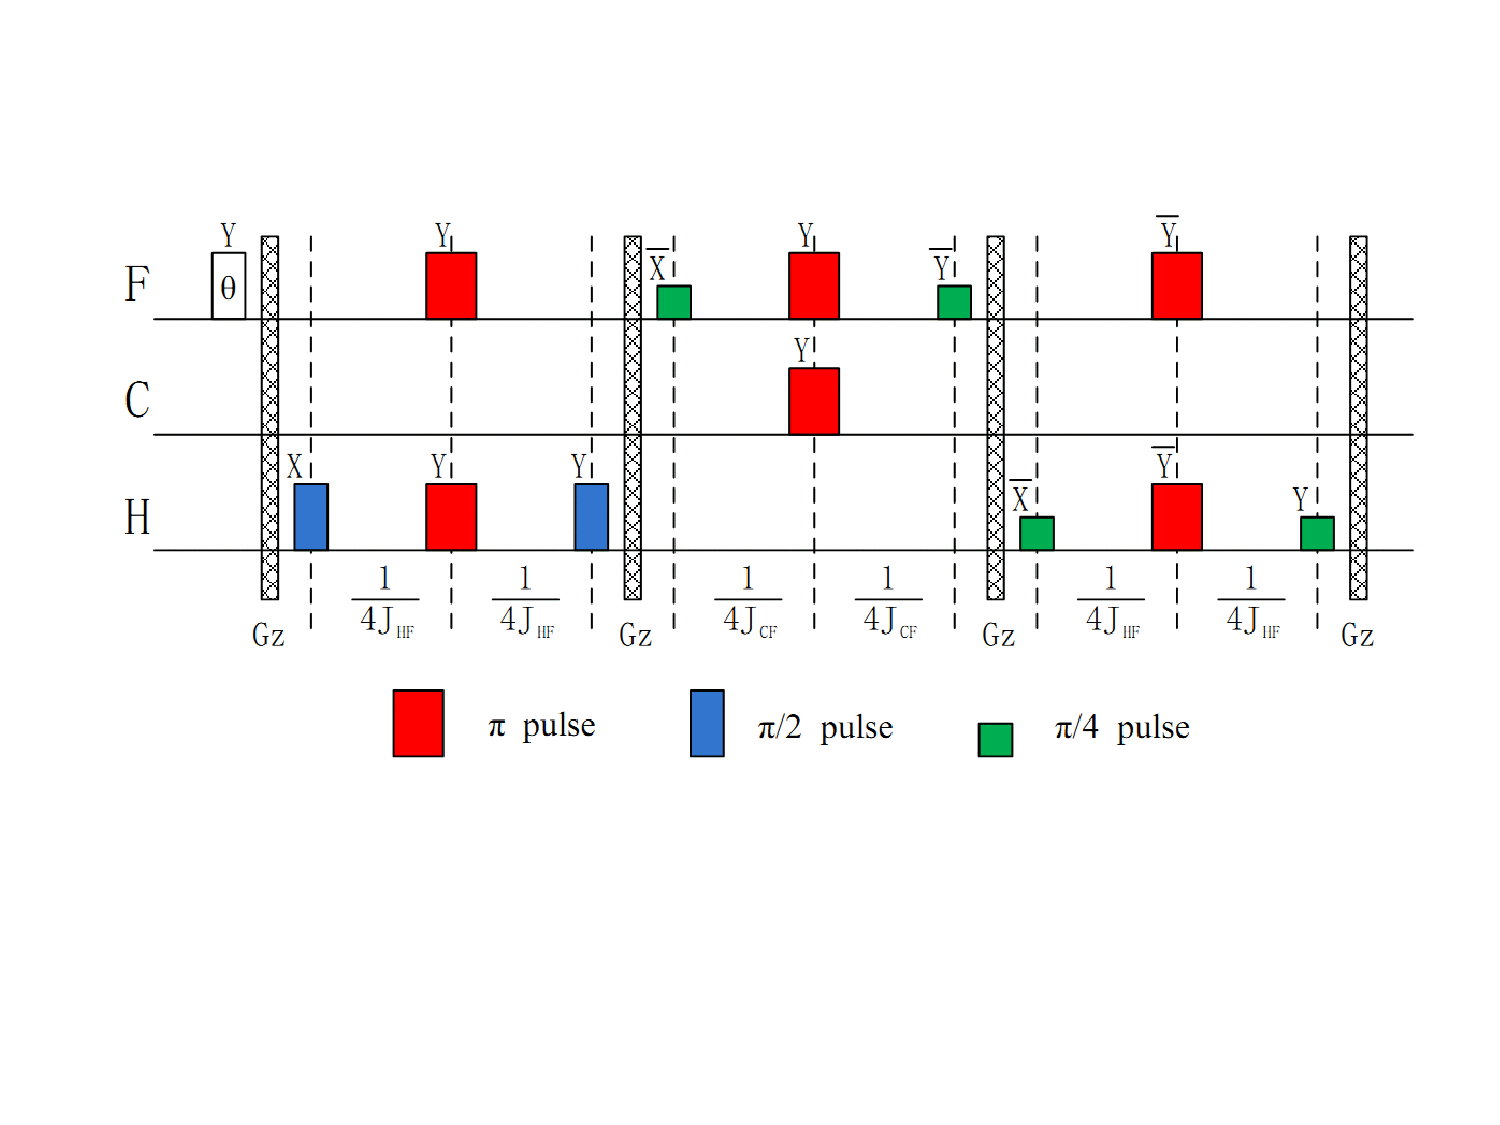
\includegraphics[width= 0.8\columnwidth]{figures/nmrdymini.pdf}
              \caption{实验上制备PPS的脉冲序列。初始的旋转角度为$\theta=0.64\pi$,且$\texttt{X}(\overline{\texttt{X}}$分别代表
              绕$\hat{x}$($-\hat{x}$, $\hat{y}$, $-\hat{y}$)轴的旋转。$G_z$则是用来消除由单比特旋转和自由演化带来的相干项。自由演化时间$\frac{1}{4\text{J}_{\text{HF}}}$和$\frac{1}{4\text{J}_{\text{CF}}}$
              分别为5.252 ms 及1.286 ms。}\label{nmrdymini}
            \end{center}
 \end{figure}

 (a) \emph{初态制备}

 在制备基态$\left\vert \phi_{0} \right\rangle$之前,我们首先要从热平衡态初态制备PPS。在该样品中,热平衡态的形式为
 \begin{equation}
\rho_{ther}=\sum\limits_{i=1}^3 \gamma_i I_z^i,
\end{equation}
其中$\gamma_i$是核自旋的旋磁比。特别地,$\gamma_\texttt{H}=4$ 且$\gamma_\texttt{F}=3.7$,这会影响到我们利用空间平均法制备PPS时
第一个单比特旋转的角度。而我们要制备的PPS形式为
\begin{equation}\label{ppsform}
\rho_{000}=\frac{1-\epsilon}{8}\mathbb{{I}}+\epsilon \left\vert 000 \right\rangle \left\langle000\right\vert,
\end{equation}
$\epsilon \approx 10^{-5}$是系统的极化度,${\mathbb{{I}}}$是$8\times8$的单位阵。单位阵当然对我们的NMR实验没有影响,因此可以忽略掉。

从热平衡态出发制备PPS的脉冲序列参见图\ref{nmrdymini},其中$G_z$表示$\hat{z}$方向的梯度场,用来摧毁由单比特旋转及自由演化带来的相干项。
在得到PPS后,我们施加一个GRAPE脉冲来得到初态$\left\vert \phi_{0} \right\rangle$,其脉宽为10 ms,且保真度高于0.995。为了衡量我们实验上得到的初态精度,我们进行了
一个完整的密度矩阵重构。目标密度矩阵$\rho_{target}$与实验得到的密度矩阵$\rho_{exp}$之间的保真度大小为
\begin{eqnarray}
F(\rho_{target}, \rho_{exp})&\equiv& \texttt{Tr}(\rho_{target}\rho_{exp})/\sqrt{(\texttt{Tr}(\rho_{target}^2)\texttt{Tr}(\rho_{exp}^2)} \nonumber \\
&\approx & 0.95.
\end{eqnarray}
关于两个密度矩阵之间的细节比较可以参考图\ref{nmrdyminiden}。

 \begin{figure}[htbp]
            \begin{center}
              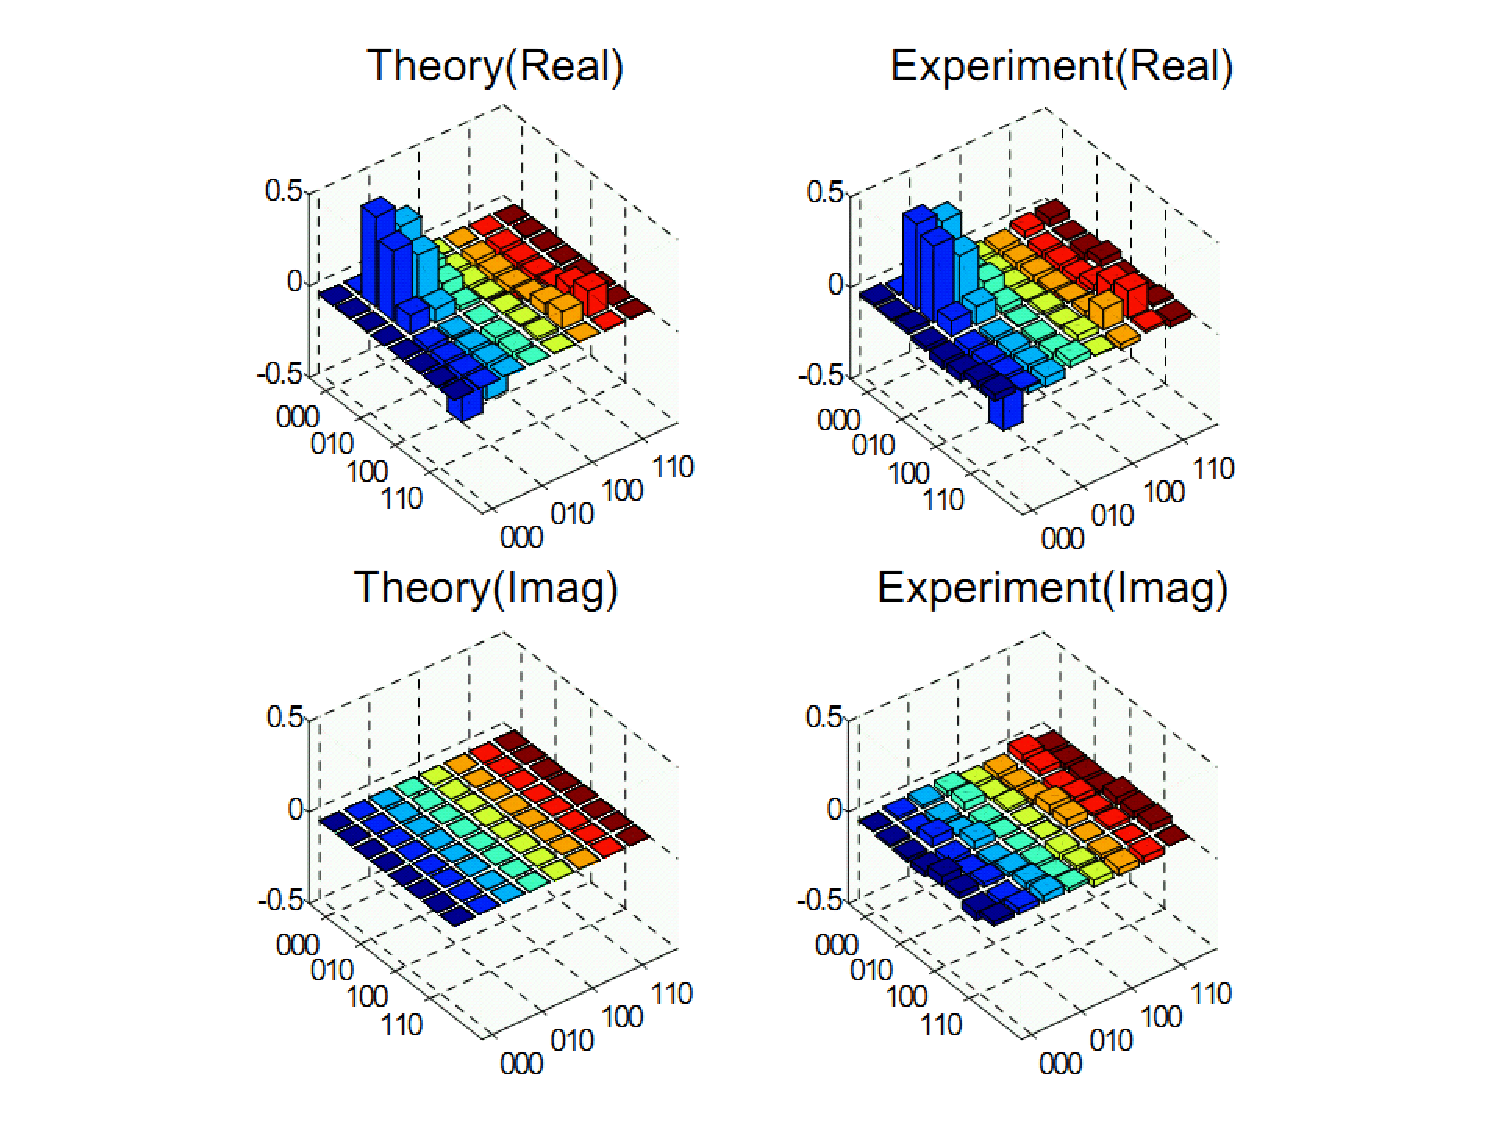
\includegraphics[width= 0.8\columnwidth]{figures/nmrdyminiden.pdf}
              \caption{实验上得到的初态$\left\vert \phi_{0} \right\rangle$对应的密度矩阵与理论密度矩阵之间的比较。理论上的结果是基于8个点的离散计算出来的。这里同时给出了密度矩阵的实部和虚部。}\label{nmrdyminiden}
            \end{center}
 \end{figure}

 (b) \emph{动力学演化}

整个反应过程被划分为25个相等的时间间隔,每一个时间间隔为$\delta t$。对于第$m$个时间间隔来说,其幺正算子为
\begin{equation}
U_m\approx V_{\delta t/2}{E}_{\delta t/2}(t_m)U_{QFT}T_{\delta t}U_{QFT}^{\dagger}{E}_{\delta t/2}(t_{m}){V}_{\delta t/2},
\end{equation}
$U_{QFT}$表示QFT操作算符,其他操作算符的定义则为${V}_{\delta t/2}\equiv e^{-\frac{i}{\hbar}{V}\frac{\delta t}{2}}$,${T}_{\delta t} \equiv e^{-\frac{i}{\hbar}{T}\delta t}$, ${E}_{\delta t/2}(t_m)\equiv e^{\frac{i}{\hbar}\varepsilon(t_{m-1}+\delta t/2) e q\frac{\delta t}{2}}$。
所有的$V$, $T$和 $q$都是各自对角表象中的形式。

在进行了8个点的势能函数曲线离散化之后,我们得到的$V_{\frac{\delta t}{2}}$, $T_{\delta t}$ 和 $q$的对角元为
\begin{eqnarray}
  {V}_{diag} =&&(293.78,-0.10,1.85,5.41,\nonumber\\
             &&  5.46,2.02,0.18,305.44)\times 10^{-3};\nonumber\\
  {T}_{diag} =&&(0,0.91,3.63,8.16,\nonumber\\
&&  14.51,8.16,3.63,-0.91)\times 10^{-3};\nonumber\\
  {q}_{diag} =&&(-1.51,-1.08,-0.65,-0.22,\nonumber\\
&&  0.22,0.65,1.08,1.51).
\end{eqnarray}
为了实现$E_{\frac{\delta t}{2}}$算子,我们还需要对含时的外加电场进行离散化。由于反应过程被分为了25步,我们也把外加电场利用25个点离散
\begin{equation}
\varepsilon(t)=[0.05,0.42,0.85,1,...1,0.85,0.42,0.05] \times 10^{-3}.
\end{equation}

从上面的分解形式看,$U_m$中的每个操作都可以通过设计的射频脉冲序列来实现,而QFT的拆解方式可以参见图\ref{qft}。虽然可以这么做,这种拆解势必需求
非常长的逻辑门操作时间及非常复杂的脉冲序列。据计算,整个序列的演化时间超过两秒,已经超过了系统的退相干时间。这种实现途径必然会累加大量的实验误差,并产生
严重的退相干效应。为了克服这个问题,我们在实验上选择了GRAPE脉冲来精确实现所需的幺正演化。

\begin{figure}[htbp]
            \begin{center}
              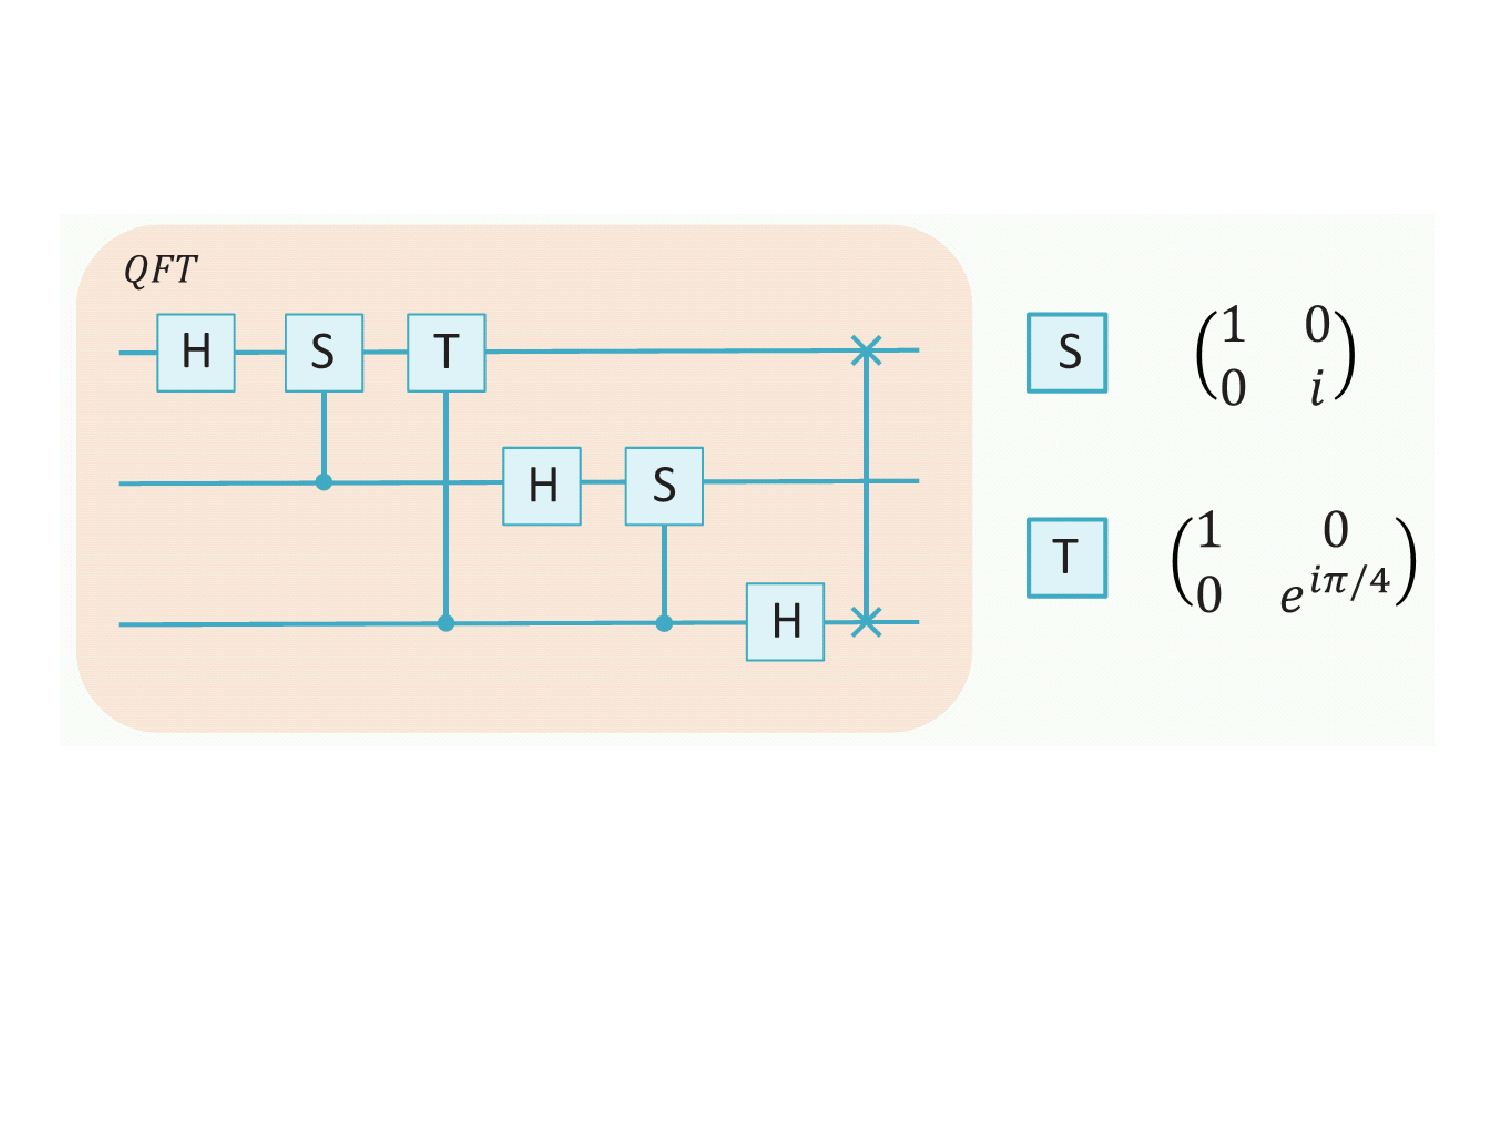
\includegraphics[width= 0.8\columnwidth]{figures/qft.pdf}
              \caption{执行QFT的网络图。H是一个Hadamard操作,S,T则是如右边所示的相位门操作。实点表示的是控制相位门。
              可以看出,这个序列已经比较复杂。}\label{qft}
            \end{center}
 \end{figure}

对于演化算子
\begin{equation}
U(t_j, 0) = \prod_{m=1}^{j}U_m,
 \end{equation}
 我们利用一个GRAPE脉冲把它们整体打包。由于实验上一共分了25步,我们一共需要25个GRAPE脉冲,每一个的保真度
 都高于0.99。计算得到的所有GRAPE脉冲的脉宽都在10ms到15ms之间。作为一个示例,图\ref{nmrdymgrape}给出了一个实现
 $t=0$ 到$t_7=7\delta t$之间的演化的GRAPE脉冲,该脉冲同样也包含了初态制备的操作算子以及后面要提到的读出用算子$R$。
 这个脉冲被分为了750小片,且保真度高于0.99。

 \begin{figure}[htbp]
            \begin{center}
              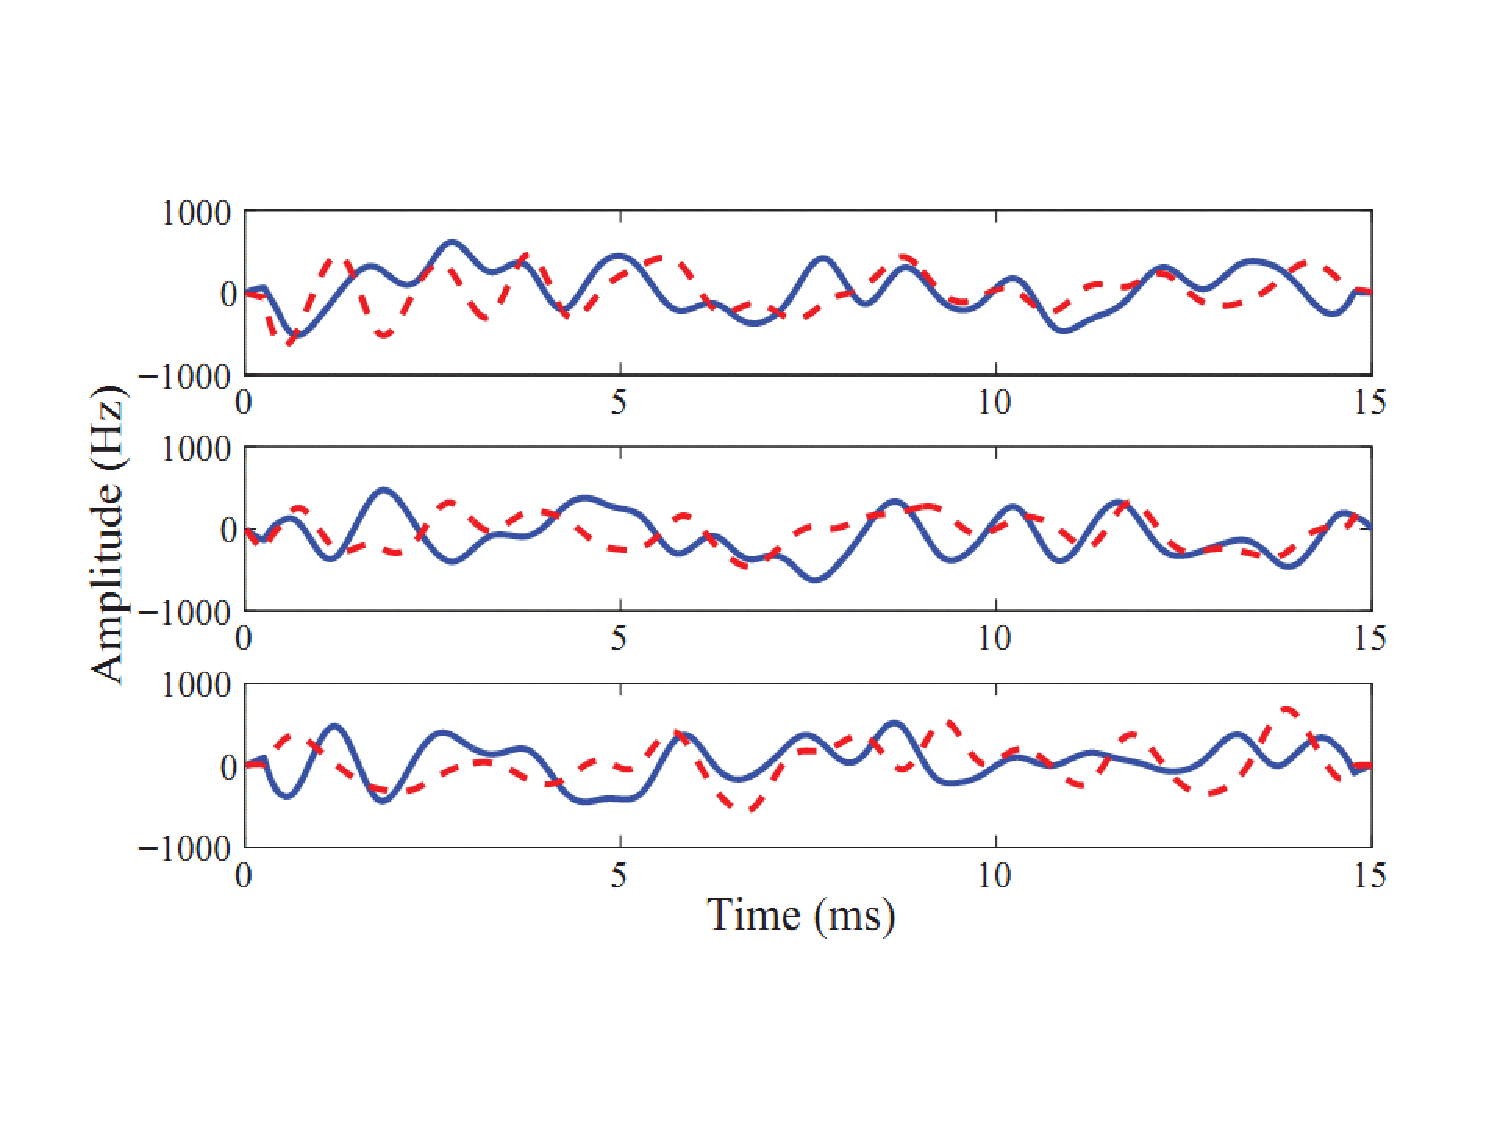
\includegraphics[width= 0.8\columnwidth]{figures/nmrdymgrape.pdf}
              \caption{化学反应中从$t=0$到$t_7=7\delta t$之间演化算子的GRAPE脉冲。从上到下分别表征的是
              加在F通道,C通道及H通道上的含时射频脉冲。蓝色的实线和红色的虚线分别表示$\hat{x}$方向以及$\hat{y}$方向的脉冲能量。}\label{nmrdymgrape}
            \end{center}
 \end{figure}

  (c) \emph{交叠度测量}

 为了衡量化学反应过程模拟的好坏,我们有必要时时监控当前的反应物及产物的比率。为了实现这个目的,我们在25步中每一步
 $t_m=m\delta t$都要测量两个交叠度$C(| \psi({t_m}) \rangle,| \phi_{0} \rangle)$ and $C(| \psi(t_{m}) \rangle,| \phi_{1} \rangle)$。
 一般来说,我们需要在每一个时间点上都进行完整的量子态重构,但这样做的复杂度非常高,而且会产生很多的多余信息。下面介绍我们在测量中用到的简化的对角化方法。

 不失一般性,考虑如何测量交叠度$C(| \psi_{7} \rangle,| \phi_{0} \rangle)$
 \begin{equation}
C(| \psi(t_{7}) \rangle,| \phi_{0} \rangle)=| \langle\phi_0|\psi(t_7)\rangle |^2=\texttt{Tr}[\rho(t_7) \rho_0],
\end{equation}
其中 $\rho(t_7)=\left\vert \psi(t_{7} \right\rangle\left\langle \psi(t_{7}) \right\vert$且$\rho_0=\left\vert \phi_{0} \right\rangle\left\langle \phi_{0} \right\vert$。假设$R$是一个算子,且能够使$\rho_0$
对角化 $\rho_0'=R \rho_0R^{\dagger}$。那么
\begin{eqnarray}
\texttt{Tr}[\rho(t_7) \rho_0]=\texttt{Tr}[R\rho(t_7) R^{\dagger}R \rho_0R^{\dagger}]=\texttt{Tr}[\rho'(t_7) \rho_0'],
\end{eqnarray}
$\rho'(t_7)=R \rho(t_7)R^{\dagger}$。明显可以看出,只有$\rho'(t_7)$的对角项会对计算$\texttt{Tr}[\rho'(t_7) \rho_0']$的结果产生贡献。
现在我们只需要测量$\rho'(t_7)$的对角项,也就是布居度就可以了。当然,一般来说$R$的形式是无规则的,也很难拆解,但利用GRAPE脉冲就可以
轻松解决这个问题。

 \begin{figure}[htbp]
            \begin{center}
              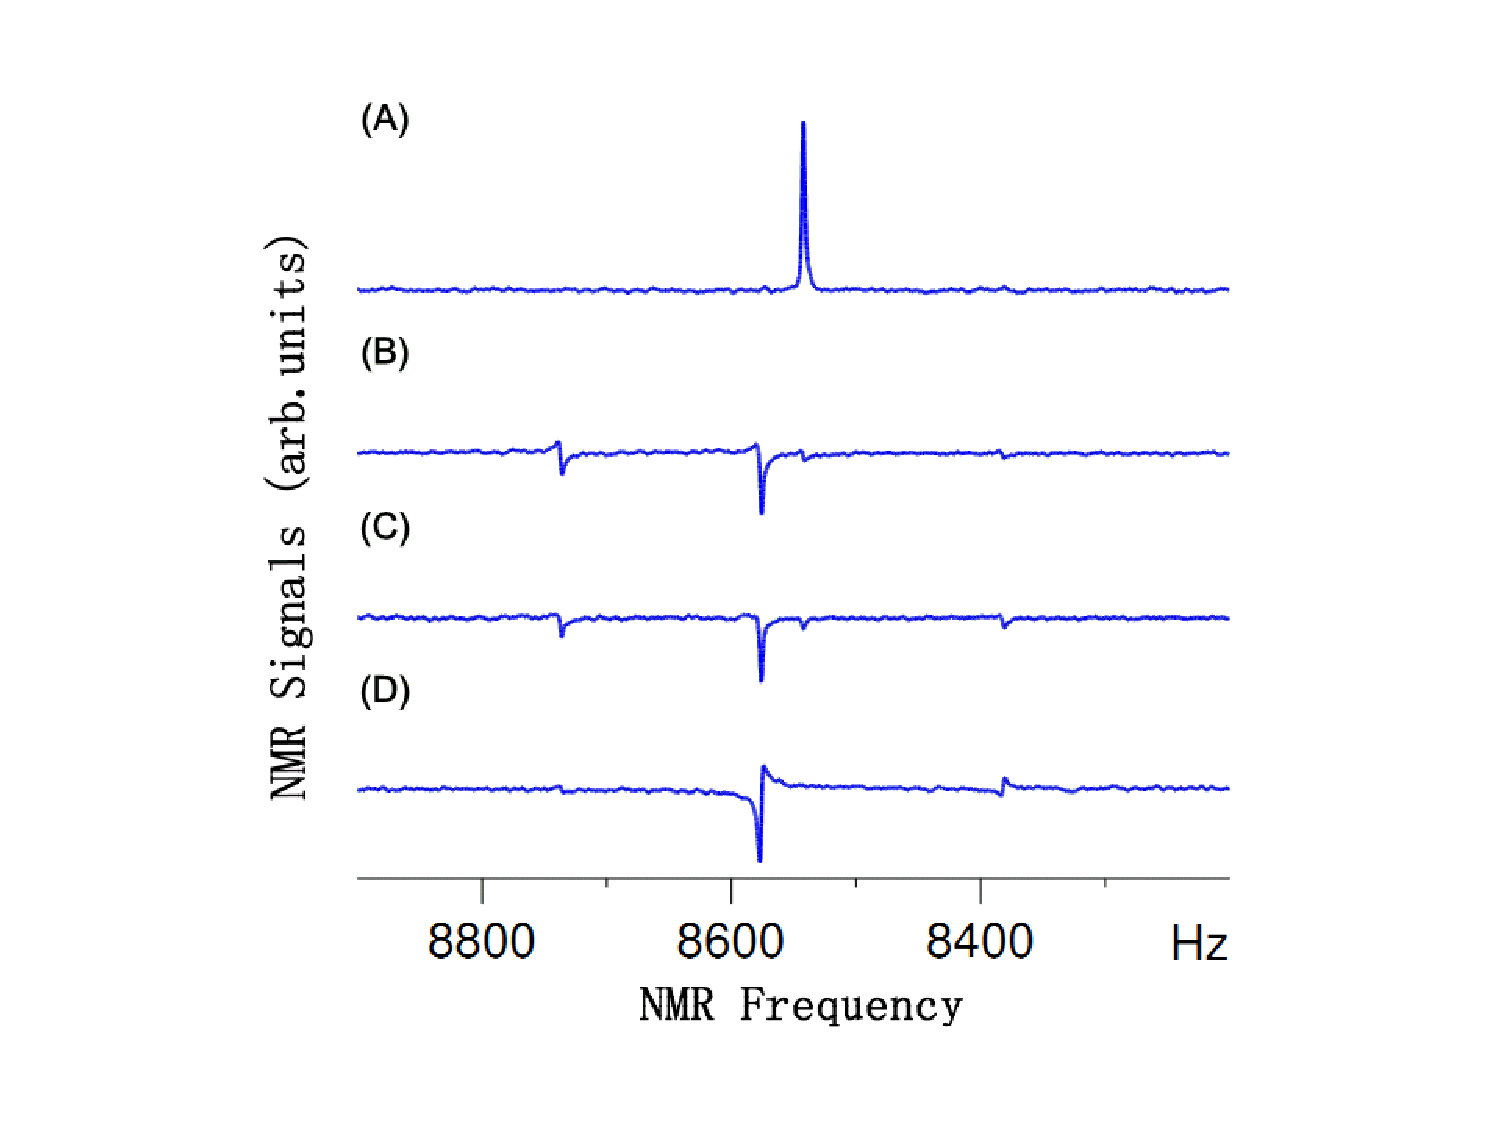
\includegraphics[width= 0.8\columnwidth]{figures/nmrdymspec.pdf}
              \caption{施加了图\ref{nmrdymgrape}所示的GRAPE脉冲后,用来测量当前密度矩阵布居度的NMR谱图。(a) 在PPS $\left\vert 000 \right\rangle$
              后加$R_y(\pi/2)$观测脉冲后的谱图,用作后面积分的基准。(b)-(d) 在$^{19}$F, $^{13}$C 以及 $^1$H上执行了GRAPE脉冲以及相应的$R_y(\pi/2)$脉冲后的谱线。注意所有的谱线都是通过SWAP门转移到$^{13}$C
              通道上进行观测的。每一条谱线的积分强度会给出$\rho'(t_7)$中两个布居度之差的值。}\label{nmrdymspec}
            \end{center}
 \end{figure}

 在执行了图\ref{nmrdymgrape}所示的GRAPE脉冲后,相应的三个用来读出当前密度矩阵布居度的NMR谱线如图\ref{nmrdymspec}显示。比如,对于
 图\ref{nmrdymspec}(c)所示的$^{13}$C的观测,从左到右的四条峰分别对应$P(5)-P(7)$, $P(6)-P(8)$, $P(1)-P(3)$及$P(2)-P(4)$,$P(i)$则是$\rho'(t_7)$第
 $i$个布居度的值。实验上,这四条峰的积分强度(与PPS的信号强度比较)分别为$-0.098$, $-0.482$, $-0.089$ 和 $-0.071$,而对应的理论值为
 $-0.047$, $-0.501$, $-0.114$ 和 $-0.041$。可以看出,实验结果和理论是比较接近的。同时,结合$^{19}$F和 $^1$H的谱图以及
 归一化条件$\sum_{i=1}^{8} {P}({i})=1$,我们可以求解所有的8个布居度,也就可以计算得到$C(| \psi(t_{m} \rangle,| \phi_{1} \rangle)$。
 对于第7次循环来说,理论和实验的交叠度大小分别为0.535和0.529,其他情况的交叠度计算可以类似得到。

 至于要把${}^{1}$H 和${}^{19}$F通道的信号通过SWAP门转移到 $^{13}$C上,是因为我们的样品是未标记的。在样品中,大概只有
 $1\%$的分子中包含$^{13}$C的核自旋,也就是有NMR信号。如果不加SWAP门的话,${}^{1}$H 和${}^{19}$F核自旋的信号将被大量的含${}^{12}$C同位素的分子支配。

 当然,以上的过程只是简化读出的过程。为了度量理论和实验的差别,我们对$t=t_f$时的末态密度矩阵进行了完整的量子态重构(图\ref{nmrdymcurve}(b))。由于我们计算出的GRAPE脉冲保真度已经高于0.995,因此实验密度矩阵
 $\rho_{\text{exp}}(t_f)$与理论结果$\rho_{\text{theory}}(t_f)$非常接近。它们之间的保真度为$F[\rho_{\text{theory}}(t_f),\rho_{\text{exp}}(t_f)]=0.957$。
 图\ref{nmrdymcurve}(c)则给出了实验上得到的反应物和产物的即时比例,可以看到反应物比例是随着时间的增加逐渐减少的,而产物的比例是逐渐增加的,并最终达到
 $77\%$的大小。至此,我们可以说已经完成了该异构反应的量子模拟。

 由于我们选择了高精度的GRAPE脉冲来完成这个实验,而且总的实验时间也仅仅为30ms左右,因此系统的退相干影响是非常小的。理论和实验结果之间的微小差别
 可以归结于GRAPE脉冲的不完美性,射频场以及静磁场的不均匀性等。

  \begin{figure}[htbp]
            \begin{center}
              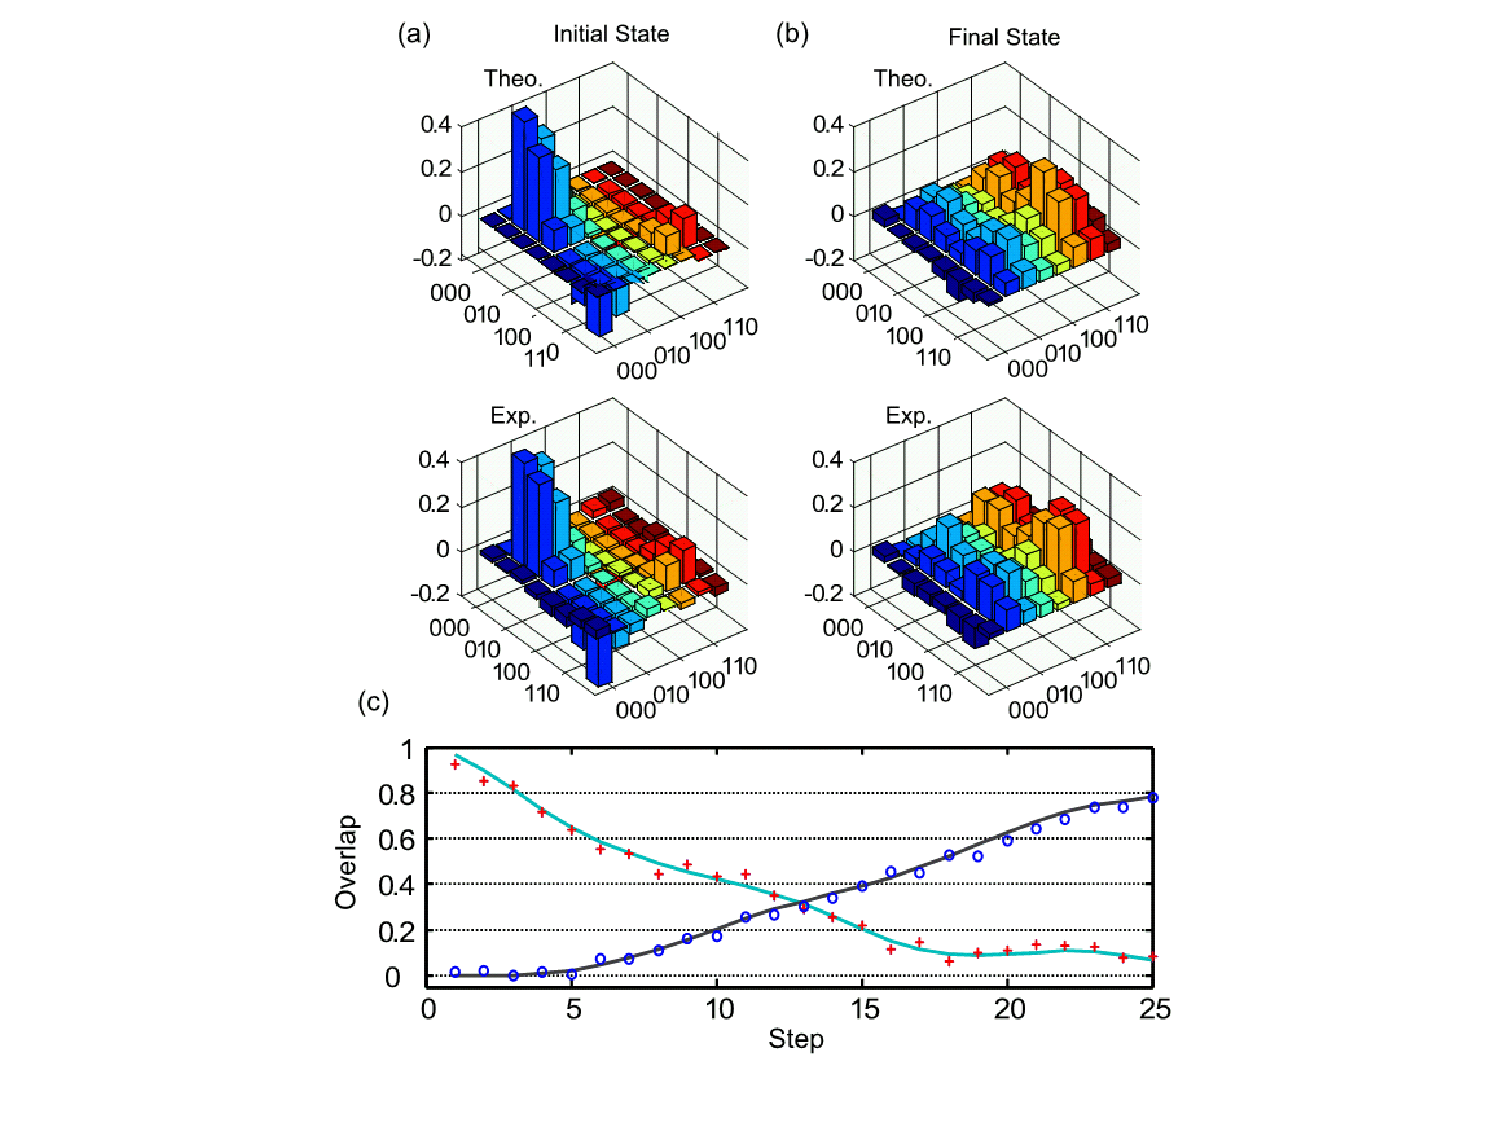
\includegraphics[width= 0.7\columnwidth]{figures/nmrdymcurve.pdf}
              \caption{(a),(b) 反应中的初态以及末态密度矩阵的实验重构结果和理论结果比较。上栏显示的是理论结果,下栏则为实验结果。(c) 即时测量的25步中每步结束后反应物和产物的比率。红色的加号表示的是当前反应物比例
              C($\left\vert \psi(t_j)\right\rangle$,$\left\vert \phi_{0} \right\rangle$),而蓝色的圆圈则是当前的产物比例C($\left\vert \psi(t_j) \right\rangle$,$\left\vert \phi_{1} \right\rangle$)。可以看出,生成物和产物的变化都和理论曲线符合的很好,也表征我们成功模拟了
              该化学反应。}\label{nmrdymcurve}
            \end{center}
 \end{figure}

本节的工作已发表在Phys. Rev. Lett. 107, 020501 (2010)\cite{dynamical}上。同时,由于我们在量子化学模拟领域完成的这些实验工作,我们还接受到了包括
Phys. Chem. Chem. Phys. Perspective以及Phil. Trans. R. Soc. A等杂志的综述性文章的约稿邀请。目前,这些邀稿文章已经在投,其中后者已被接收\cite{invited1},前者仅
需简单修改即可发表\cite{invited2}。

\section{Heisenberg模型本征能级问题的求解}

\subsection{本征能级求解的理论方案}

在量子模拟中,最有挑战性的问题之一是所谓的本征能级求解问题。待求的哈密顿量可以是经典的,也可以是量子力学的。
这种问题的目的就是在给定哈密顿量后,求解得到其本征值和本征态。一般来说,每一个量子线路\cite{heisen1},甚至热态\cite{heisen2,heisen3},都可以编码为
特定哈密顿量的本征能级问题。遗憾的是,这种本征能级问题的求解并没有已知的经典或量子算法可以适用。

当哈密顿量涉及到物理或化学领域时,由于它们的哈密顿量经常展现出特殊的结构和对称性,就产生了一些近似处理
方法,比如利用试探态$|\Psi_T \rangle$来近似基态。但是,当试探态$|\Psi_T \rangle$和目标态$|e_0 \rangle$的交叠度很小,也就是
$F \equiv \langle e_0 |\Psi_T \rangle$的值很低时,这种试探态的方法就会失效。比如,在经典多体问题中,如果我们选择的试探态的保真度只有0.01,
那么它作为基态的近似是非常不精确的,也不适合做经典计算的初态。相反地,在量子计算中,同样的试探态则可以作为有效的输入,因为
我们只要把基态投影过程\cite{lq7}重复大概$O(100)$次就可以了。这在计算复杂度上是有效的,特别在多体哈密顿量的Hilbert空间是指数增长的情况下。

我们选择的模型是含外磁场的Heisenberg自旋模型,研究目标主要为:确定基态的本征值,即本征能量;从保真度为0.5的试探态出发,
最大化或者说纯化该试探态,使其尽可能的接近基态。对于第一个目标,我们利用了改进后的迭代PEA算法,并把精度
提高到$10^{-5}$。然后,我们通过态过滤的方法计算基态与末态之间的保真度,以达到第二个目标。在实验上,我们特别选择了三个不同的外场强度,分别是
$h =0$,$h =0.75h_c$,$h =1.25h_c$。其中$h_c$表征的是相变点,也就是基态与第一激发态的交叉点的外磁场强度。

 \begin{figure}[htbp]
            \begin{center}
              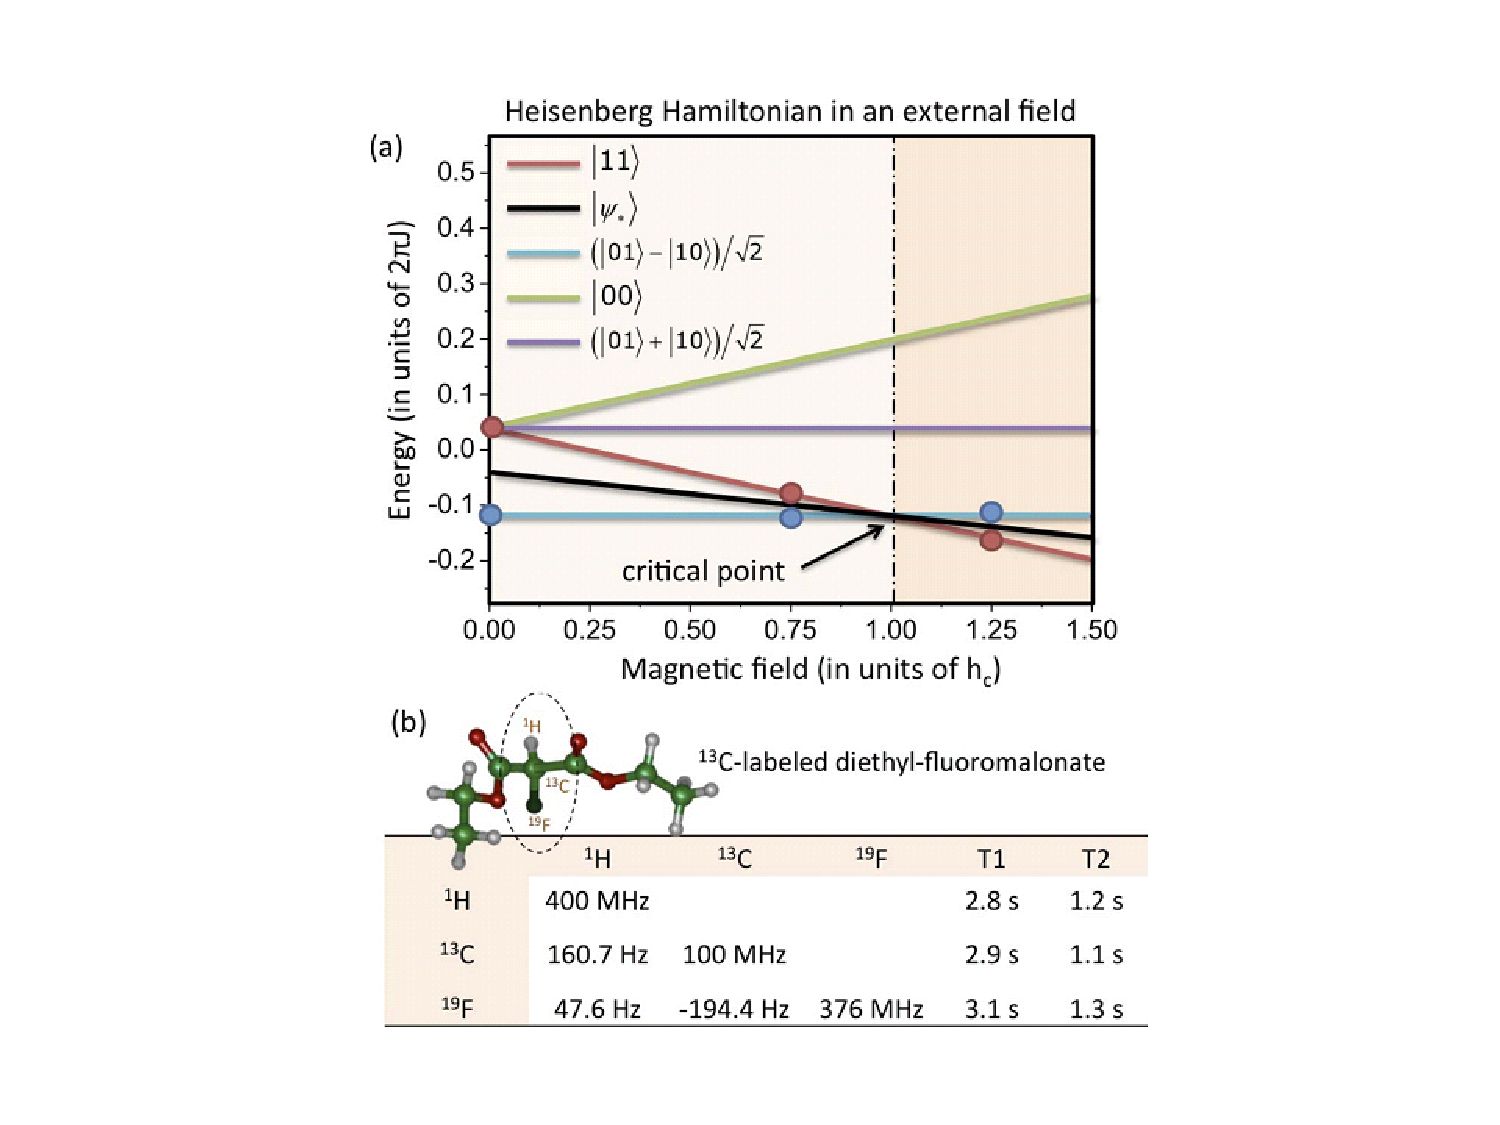
\includegraphics[width= 0.7\columnwidth]{figures/heisen1.pdf}
              \caption{(a)Heisenberg模型的哈密顿量中外磁场强度与本征值之间的关系。我们选择的试探态
              $|\Psi\ast\rangle \equiv|\Psi(-\pi/4,\pi/2)\rangle$(黑线)是另外两个本征态之间的线性组合(蓝线和红线)。(b)
              实验用到的3 qubit样品Diethyl-fluoromalonate 及其参数。}\label{heisen1}
            \end{center}
 \end{figure}

含外加$\hat{z}$方向磁场的Heisenberg模型哈密顿量为
 \begin{equation}
H = J(I_x^aI_x^b+I_y^aI_y^b+I_z^aI_z^b)+h(I_z^a+I_z^b).
\end{equation}
我们可以选择的试探态并没有特殊的限制,理论上只要不与基态正交的态都可以用作试探态。对于更一般的系统,我们要求试探态满足如下两个性质:
(1) 它包含一个或更多的可调参数,使得可以最小化$\langle H\rangle$,通常来说这个过程不会产生精确的基态;
(2) 它可以只包含哈密顿量的本征态张成的矢量空间的一部分。比如,对于上面的哈密顿量模型,试探态
 \begin{equation}
|\Psi(\theta,\phi)\rangle = \frac{1}{\sqrt{2}}|\theta\rangle+\frac{1}{\sqrt{2}}|\phi\rangle
\end{equation}
即满足上面的两个条件。一般来说,对于给定的$(J, h)$最优的态是不同的,但我们发现,
在上面的哈密顿量形式下,$|\Psi\ast\rangle \equiv|\Psi(-\pi/4,\pi/2)\rangle$是可以对所有的$h$以及$J>0$最小化
$\langle H\rangle$的。这个最优化的态也恰好包含了哈密顿量四个本征能量中的两个,而其保真度和基态
$|e_0\rangle $之间的保真度恰好为$50\%$。当然,我们还是要强调,即使初始保真度很低,只要后面哈密顿量本征值的
谱线可以从噪声中分开,那么这个方案依然是有效的。

在算法开始时,系统qubit被制备到试探态$|\Psi\ast\rangle = \sum_k a_k |e_k\rangle$,而辅助qubit则被制备到
$(|0\rangle+|1\rangle)/\sqrt{2}$。对于不同的时间$t$,执行控制演化操作$U(t) = e^{-iHt}$。此时,整个体系的末态将变为
\begin{equation}
\frac{1}{\sqrt{2}}\sum_k a_k(|0\rangle+e^{-i\omega_k t}|1\rangle)|e_k\rangle ,
\end{equation}
其中$\omega_k = E_k$。此时辅助qubit的约化密度矩阵形式为
\begin{equation}
\rho_{probe}(t)=\frac{1}{2}\left(
                             \begin{array}{cc}
                               1 & \sum_k |a_k|^2e^{i\omega_k t}  \\
                               \sum_k |a_k|^2e^{-i\omega_k t} & 1 \\
                             \end{array}
                           \right).
\end{equation}
从这个形式可以看出,本征值的信息就被包含在该矩阵的非对角项中,而对非对角项在不同时间点的信号进行经典傅里叶分析就可以得到
本征值$\omega_k$和交叠度$|a_k|^2$。为了得到高精度的$\omega_k$,通常来说需要很长的时间演化。但对于该方案中选择的高对称性哈密顿量
模型来说,我们还可以利用简化过的迭代PEA算法来实现这个过程。

一旦哈密顿量的基态本征值$E_0$确定下来,我们就可以利用态过滤\cite{heisen5}等方法把基态$|e_0\rangle $
与其他的态分离开来。该方法的末态形式为
\begin{equation}
a_0 |e_0\rangle |00\ldots 0\rangle + \ldots,
\end{equation}
省略掉的部分表示此时辅助qubit所处的状态和$|00\ldots 0\rangle$正交。此时,如果我们对辅助qubit进行投影测量,
那么系统qubit塌缩到基态的概率就为$|a_0|^2$。至此,我们就成功解决了该哈密顿量的基态能级问题。

\subsection{实验实现}

实验上选择的是3 qubit样品Diethyl-fluoromalonate ,其中的三个原子核$^{19}$F, $^{13}$C, 和$^1$H
被用作3个qubit。该系统的哈密顿量为
\begin{eqnarray}
\mathcal{H}_{int}=&&\sum\limits_{j=1}^3 {2\pi \nu _j } I_z^j  + \sum\limits_{j < k,=1}^3 {2\pi} J_{jk} I_z^j I_z^k,
\end{eqnarray}
其参数可以参见图\ref{heisen1}(b)。

整个实验可以概括为三个部分:

$\bullet$ 初态制备,即把系统qubit制备到$|\Psi\ast\rangle$,而辅助qubit制备到$|0\rangle$。

$\bullet$ 利用迭代的PEA算法测量哈密顿量的本征值。

$\bullet$ 完整的量子态重构。



 \begin{figure}[htbp]
            \begin{center}
              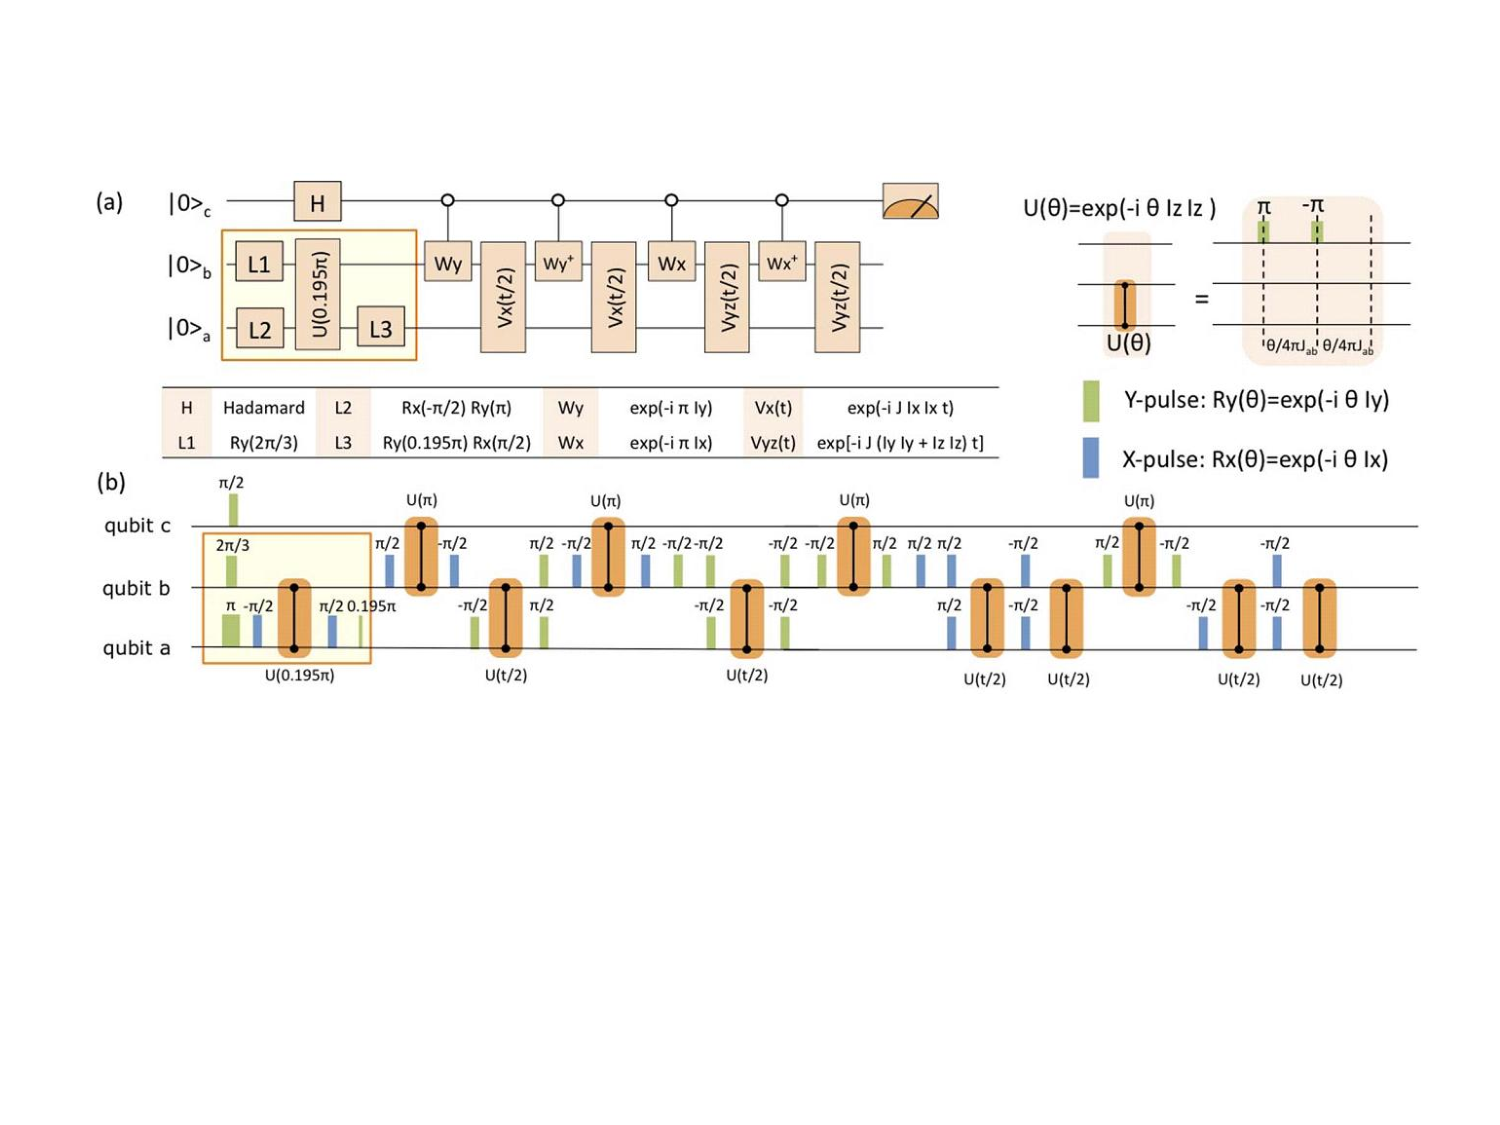
\includegraphics[width= 0.8\columnwidth]{figures/heisen2.pdf}
              \caption{(a)实验上用的量子网络图。方格标记出来的部分用来把系统qubit制备到初态$|\Psi\ast\rangle$。
              (b) 对应于量子网络图的脉冲序列示意图,这里的脉冲序列是外磁场强度$h=0$时的情况的。}\label{heisen2}
            \end{center}
 \end{figure}

在初态制备中,我们首先需要制备的是PPS $|000\rangle$。这部分内容在前面的实验,比如化学动力学模拟中已经
有了非常详细的介绍,这里略过不提。从$|000\rangle$出发,我们可以把辅助qubit通过赝Hadamard操作$R_y^c(\pi/2)$转到
态$(|0\rangle+|1\rangle)/\sqrt{2}$上。系统qubit则可以通过两个单比特旋转和一个控制旋转制备到初态
\begin{equation}
|\Psi\ast\rangle = \frac{1}{2}(|01\rangle-|10\rangle) +\frac{1}{\sqrt{2}}|11\rangle.
\end{equation}

在PEA算法中,我们要实现控制$U(t)$的演化。这部分可以利用哈密顿量的对易性来实现,见图\ref{heisen2}(a)。由于Heisenberg模型的哈密顿量
 \begin{equation}
H = J(I_x^aI_x^b+I_y^aI_y^b+I_z^aI_z^b)+h(I_z^a+I_z^b)
\end{equation}
中$J$所对应的项和$h$所对应的项是对易的,我们可以把时间演化算子$T(t)\equiv e^{-iHt}$分为三个部分
 \begin{equation}
T(t) = V_x(t) V_{yz}(t) L_z(t),
\end{equation}
其中
 \begin{equation}
V_x(t) \equiv e^{-iJI_x^aI_x^bt},
\end{equation}
 \begin{equation}
V_{yz}(t) \equiv e^{-iJ(I_y^aI_y^b+I_z^aI_z^b)t},
\end{equation}
 \begin{equation}
L_z(t) \equiv e^{-ih(I_z^a+I_z^b)t}.
\end{equation}
对于这三项控制操作的具体实验实现,可以参见文章\cite{yexiao}的补充材料部分,这里限于篇幅不再详述。

 \begin{figure}[htbp]
            \begin{center}
              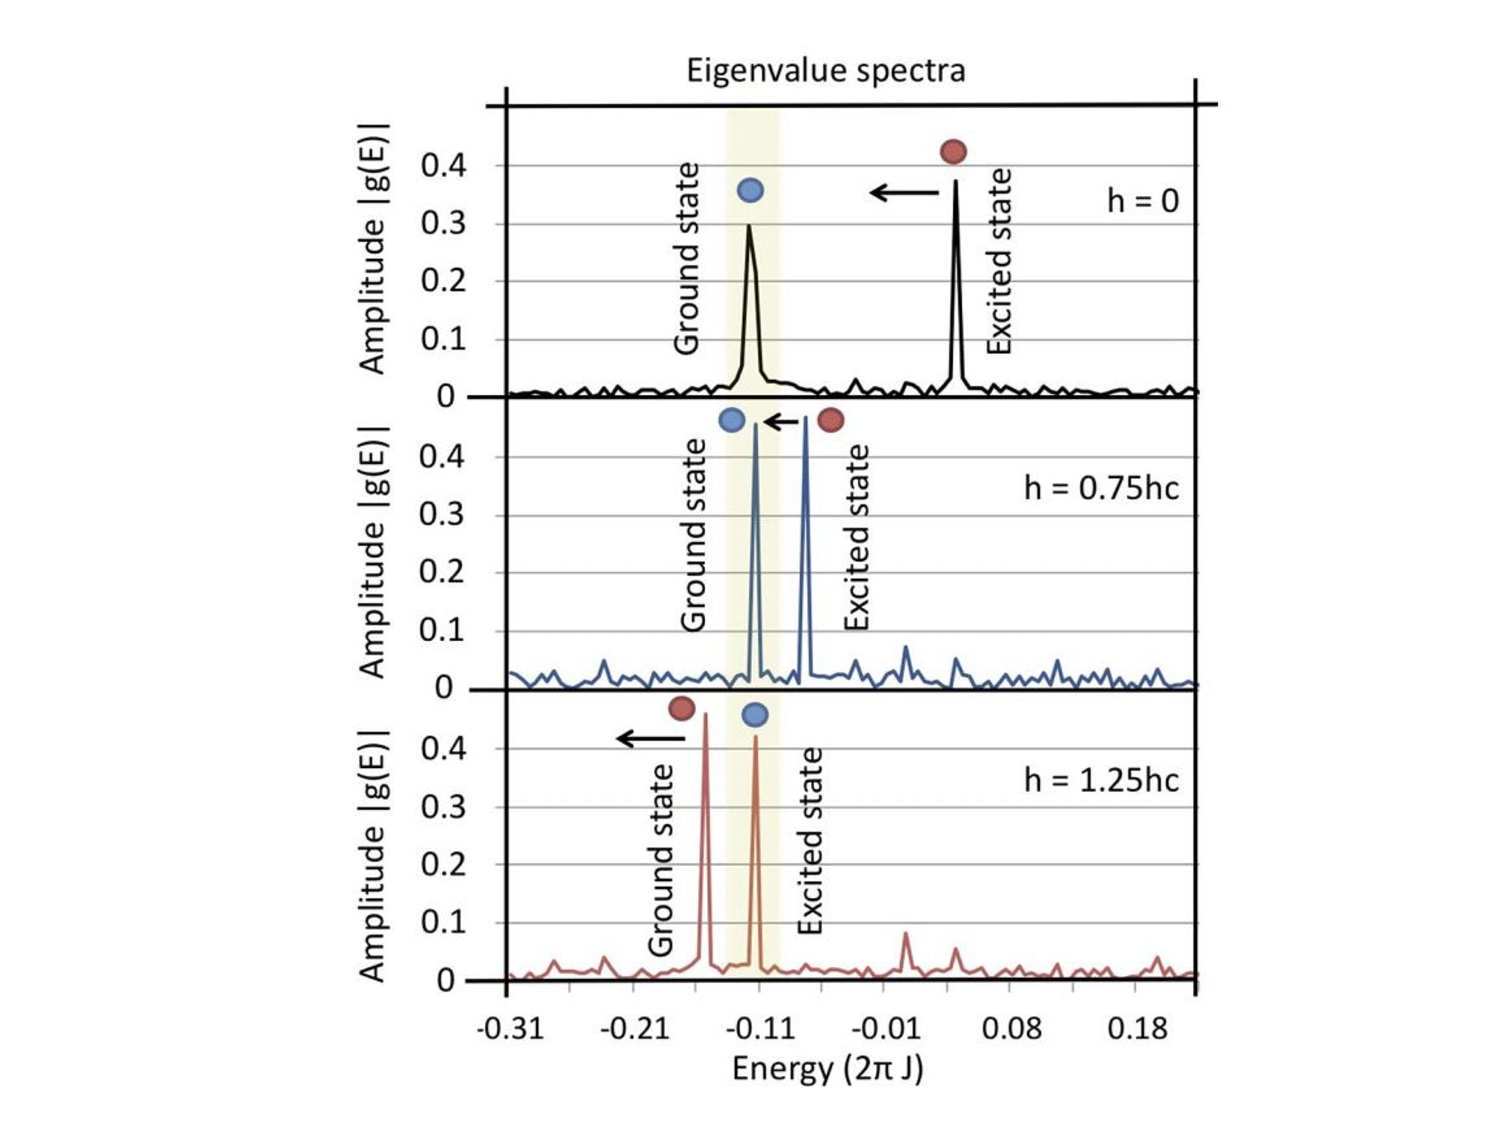
\includegraphics[width= 0.8\columnwidth]{figures/heisen3.pdf}
              \caption{对于不同的外磁场强度$h = 0,0.75h_c,1.25h_c$,Heisenberg模型哈密顿量的本征能量谱。$h_c$是基态与第一激发态简并时
              对应的外磁场强度。红色与蓝色的点分别对应于图\ref{heisen1}中的红色和蓝色代表的量子态。}\label{heisen3}
            \end{center}
 \end{figure}

在执行了PEA算法之后,我们需要对辅助qubit进行测量。定义$\rho_{probe}(t)$的非对角项为
\begin{equation}
|M_t|e^{i\phi_t}= \sum_k |a_k|^2e^{i\omega_k t}.
\end{equation}
我们可以利用NMR中的四极探测来测出其中的$\phi_t$,而NMR谱线强度的积分值则可以给出
$|M_t|$的值。然后,通过对不同的时间点实行哈密顿量演化,我们就可以利用离散傅里叶变换得到
$|M_t|e^{i\phi_t}$的频率谱。图\ref{heisen3}给出了不同的外磁场强度$h = 0,0.75h_c,1.25h_c$下的哈密顿量本征值的频率谱,每个谱图
采集了128个时间点。

为了使测量得到的本征值更加精确,我们对PEA算法进行了迭代。如果用一系列的十进制数据$\{x_1,x_2,x_3\ldots\}$来
表征本征值
\begin{equation}
\omega_k = 2\pi J\times 0.x_1x_2x_3\ldots,
\end{equation}
一旦$x_1$已知,我们就可以通过迭代的方法把$x_2$放大10倍。具体来说,只需把演化时间扩大10倍
\begin{equation}
10\times\omega_k = 2\pi J t \times x_1. 0 + 2\pi J t \times 0.x_2x_3\ldots.
\end{equation}
上式中,右边第一项是已知的,而第二项已经被放大了,可以通过PEA方法测出$x_2$。以此类推,我们可以迭代后测量$x_3$等等,直到
达到$\omega_k$所需的精度。图\ref{heisen4}给出了实验上5次迭代后的结果,可以看到本征值的误差从22$\%$提升到了约0.003$\%$。

 \begin{figure}[htbp]
            \begin{center}
              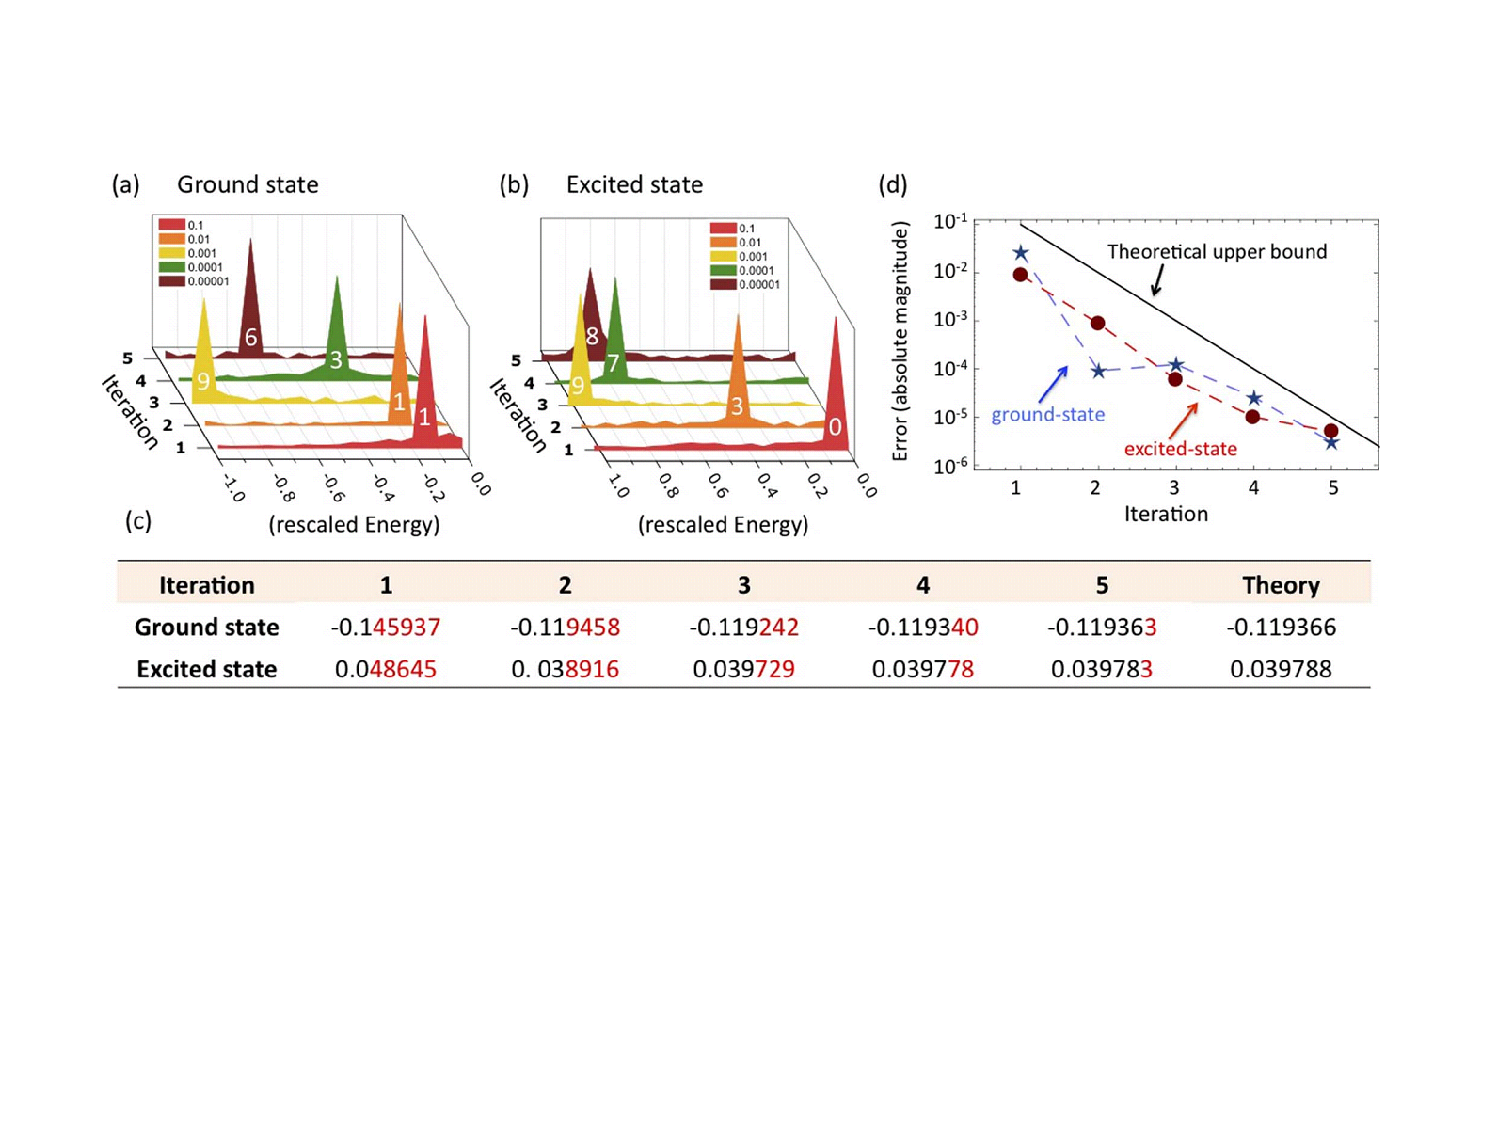
\includegraphics[width= 0.8\columnwidth]{figures/heisen4.pdf}
              \caption{为了提高测量得到的本征值的精度,我们采用了迭代的PEA算法。实验中一共采用了
              5次迭代,而达到了$10^{-5}$的精度。}\label{heisen4}
            \end{center}
 \end{figure}
 
 在利用迭代PEA算法得到了哈密顿量的两个本征值$E_0$和$E_1$后,我们可以利用和图\ref{heisen2}(a)所示的相同的脉冲序列来得到
 本征态:基态$|e_0\rangle$和第一激发态$|e_1\rangle$。不同的是,在控制$U(t)$操作$U(t) =  e^{-iHt}$中演化时间选择为
 \begin{equation}
\tau = \pi/(E_1-E_0).
\end{equation}
然后就可以得到末态
 \begin{equation}
\frac{1}{\sqrt{2}}(|e_0\rangle|0\rangle-|e_1\rangle|1\rangle).
\end{equation}
可以看出,两个本征态分别对应于辅助qubit的一组正交态,因此可以通过投影测量分开,当然在NMR上可以选择利用
完整的量子态重构技术。对于不同的外磁场强度$h = 0,0.75h_c,1.25h_c$,图\ref{heisen5}(b)-(d)给出了末态的重构结果,而(e)-(g)则给出了辅助qubit
投影测量到$|0\rangle$后系统qubit的约化密度矩阵。

 \begin{figure}[htbp]
            \begin{center}
              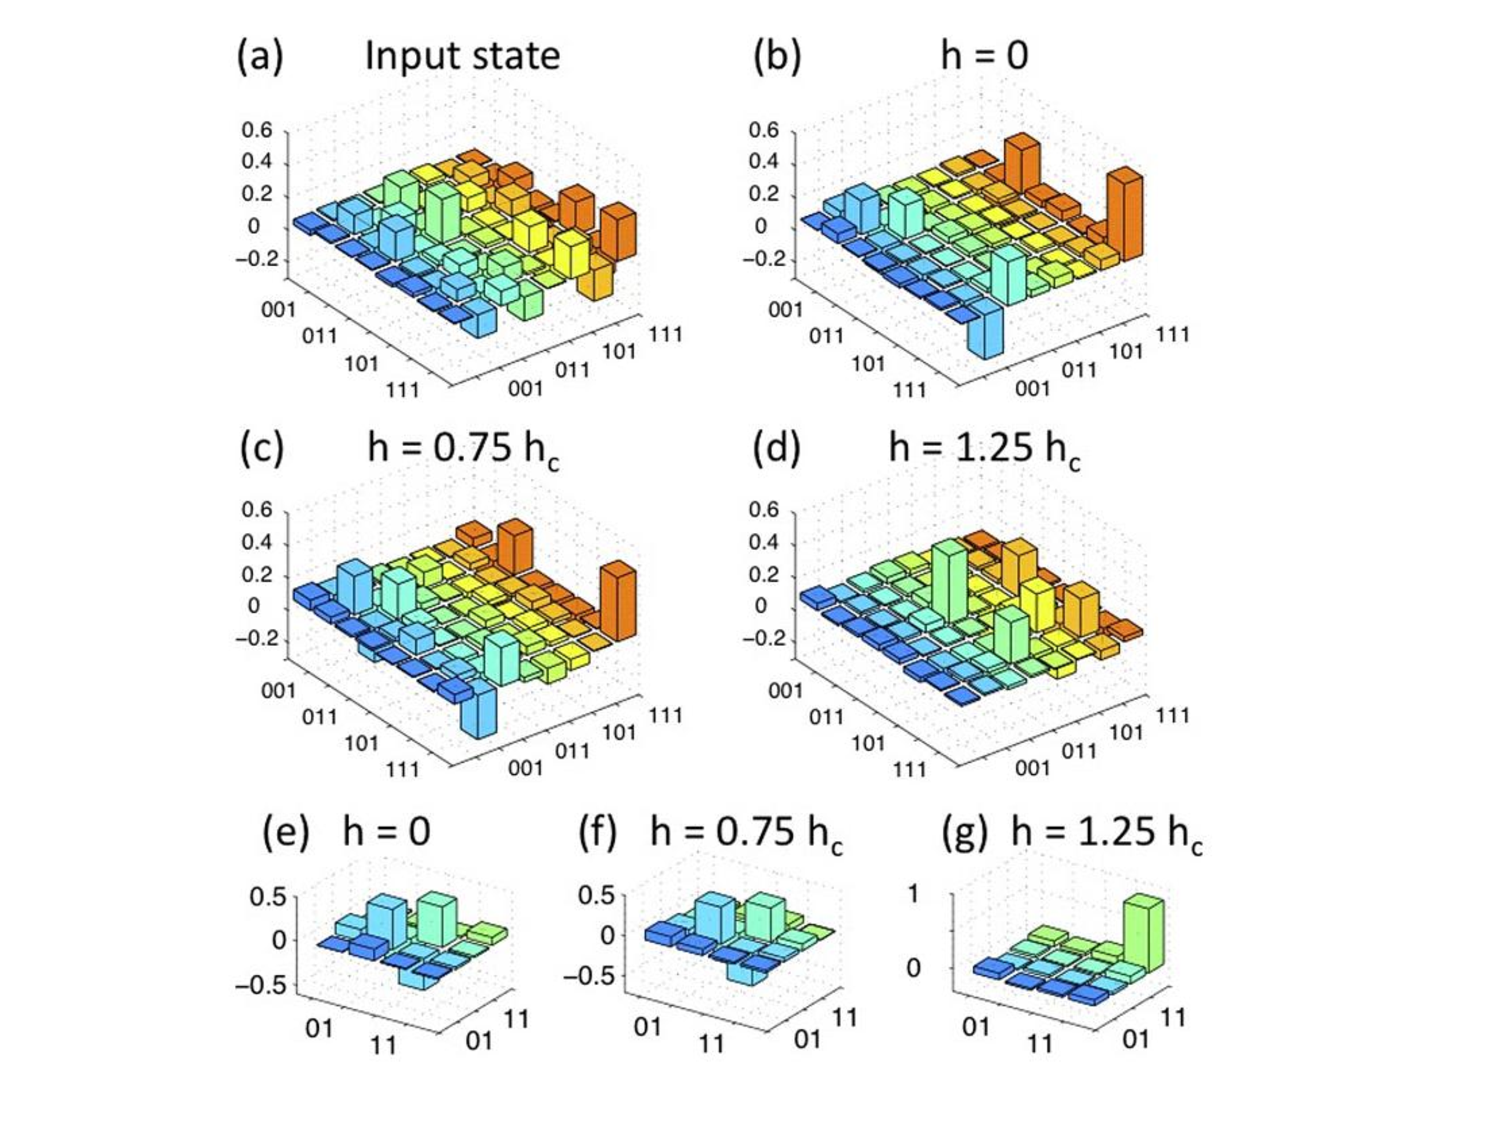
\includegraphics[width= 0.8\columnwidth]{figures/heisen5.pdf}
              \caption{从完整的量子态重构得到的实验结果。这里所有的密度矩阵仅给出了实部。(a)初态$|\Psi\ast\rangle$的密度矩阵。(b)-(d)
              对于三种不同的外磁场强度$h = 0,0.75h_c,1.25h_c$的末态密度矩阵。(e)-(g) 把辅助qubit投影到$|0\rangle$,系统qubit的约化密度矩阵。}\label{heisen5}
            \end{center}
 \end{figure}
 
 总结来说,我们利用NMR量子计算实现验证了基态能级问题的求解方法。实验上我们选择的初态和基态之间仅有
 $50\%$的交叠度,但可以通过5次迭代PEA算法把本征值的精度提升到$10^{-5}$。不仅如此,我们还高精度地得到了哈密顿量的本征态。
 这套理论不仅限于用在Heisenberg模型的哈密顿量和NMR上,也可以被扩展到更加普适的哈密顿量中,或其他的实验平台上。
 
 本节的工作已发表在Scientific Reports 1, 88 (2011)\cite{yexiao}上。

\section{小结}

在本章中,我们从理论和实验两方面回顾了量子化学模拟的重要进展。 和动辄需要上千个qubit来展示量子计算优越性的
量子算法不同,量子模拟被证明仅需30到100个qubit就可以实现这一目标。虽然今日的量子计算实验技术距离这个要求
还有一段距离,目前确实已经有了演示性的实验工作了,分别在静态分子能级模拟\cite{optics_static,static}和动态化学反应模拟\cite{dynamical}上。这些实验证明
量子模拟将是未来研究量子化学问题的一个强有力的工具,而以后的应用会更加广泛。

对当前的实验水平来说,接下来的工作主要集中在两个方面:模拟更大更复杂的分子能级以及模拟更复杂的化学反应。

在分子能级模拟方面,既然最简单也最重要的氢分子已经完成了,下一个纳入考虑的应该是水分子。在原始的理论方案中\cite{Alan_first},如果利用最简单的
STO-3G基组函数展开,模拟水分子需要8个qubit,这在一些系统比如NMR中已经是可以实现的。紧接着,一个得到分子能谱的量子算法又被提出\cite{watermo1}。作为示例,利用cc-pVDZ基组函数展开来模拟水分子基态和第一激发态能级被证明需要14个qubit。
最近又表明,如果我们选择在STO-3G基组函数展开,并只是获得水分子能谱而非基态能量的话,6个qubit就足够了\cite{watermo2}。可见,模拟水分子在近期内非常可能实验实现的。

在动力学反应模拟方面,下一步是将系统势能扩展到两维上。如果我们用16$\times$16个网格来离散化这个势场的话,则需要8个qubit,而这在很近的未来也是可行的。
当然,8个qubit后我们利用Trotter公式将得到几千个逻辑门操作,这时候就需要借助于GRAPE脉冲等精确操控技术的力量了。当然,除了基于逻辑网络的量子计算,我们也可能会选择拓扑
量子计算\cite{dymtopo}或者单向量子计算\cite{oneway1,dymoneway}等模型来实现超越一维的化学反应模拟。